%TODO
%
% diminuir o tamanho da figura dos campos snmp
% cronograma do TCC 2 (janeiro/julho)
% == Proposta ==
% retomar os objetivos
% relacionar os objetivos com IOT e Redes
% 'dado que o snmp domina faremos algo em snmp'
% quais são os requisitos, o que ela vai atender (cenário onde vai ser aplicad)
% modelo visual (motes, gateway, gerente)
% descrever cada um dos elementos do modelo
% descrever cenários de uso (agregação via gateway)
% como validar o sucesso da ideia (elaboracao do prototipo)
%
%=======================================================================
% Declarações iniciais identificando a classe de documento e
% selecionando alguns pacotes adicionais.
%
% As opções disponíveis (separe-as com vírgulas, sem espaço) são:
% - twoside: Formata o documento para impressão frente-e-verso
%   (o default é somente-frente)
% - english,brazilian,french,german,etc.: idiomas usados no documento.
%   Deve ser colocado por último o idioma principal.
%=======================================================================
\documentclass[twoside,english,brazilian]{UNISINOSmonografia}
\usepackage[utf8]{inputenc} % charset do texto (utf8, latin1, etc.)
\usepackage[T1]{fontenc} % encoding da fonte (afeta a sep. de sílabas)
\usepackage{graphicx} % comandos para gráficos e inclusão de figuras

\usepackage{tabulary}
\usepackage{pdflscape}
\usepackage{afterpage}

\usepackage{bibentry} % para inserir refs. bib. no meio do texto
\usepackage{hyperref}
\usepackage{subcaption}

\interfootnotelinepenalty=10000 % evitar a quebra de footnotes em 
								% mais de uma página

\hypersetup{
	breaklinks=true,
	unicode=true,          % non-Latin characters in Acrobat’s bookmarks
	hidelinks=true,
	linktoc=all,
	pdflang=pt-BR
}

\graphicspath{ {./images/} }

%\hypersetup{
%	pdftitle={titulo},    % title
%	pdfauthor={mateus},     % author
%	pdfsubject={subsubsub},   % subject of the document
%	pdfkeywords={kkk1} {key2} {key3}, % list of keywords
%}
%=======================================================================
% Escolha do sistema para geração de referências bibliográficas.
%
% O default é usar o estilo unisinos.bst.  Comente a definição abaixo
% e descomente a linha seguinte para usar o estilo do ABNTeX (é
% necessário ter esse pacote instalado).
%
% A vantagem do unisinos.bst é que ele permite o uso de um arquivo .bib
% seguindo as orientações tradicionais do BibTeX (veja essas orientações
% em http://ctan.tug.org/tex-archive/biblio/bibtex/contrib/doc/btxdoc.pdf).
% Entretanto, o estilo não suporta algumas citações mais exóticas como
% apud.  Para isso, use o ABNTeX, mas esteja ciente de que muitas de
% suas referências serão incompatíveis com os estilos tradicionais do
% BibTeX como plain, alpha, ieeetr, entre outros.
%=======================================================================
\unisinosbst
%\usepackage[alf]{abntcite}



%=======================================================================
% Dados gerais sobre o trabalho.
%=======================================================================
\autor{Aubin}{Mateus Rauback}
\author{Mateus Rauback Aubin}
\titulo{
Um Sistema de Gestão de Dispositivos Inteligentes 
Baseado em Protocolos de Gerência de Redes Voltado Para a 
Internet das Coisas
}
%\subtitulo{Versão \LaTeX}
\orientador[Prof.~Dr.]{Ávila}{Rafael Bohrer}
%\coorientador[Prof.~Dr.]{Lamport}{Leslie}
\local{São Leopoldo}
\ano{2013}

%% dados específicos para monografia de Graduação
\unidade{Unidade Acadêmica Graduação}
\curso{Curso de Bacharelado em Ciência da Computação}
\natureza{
Trabalho de Conclusão de Curso apresentado como requisito parcial
para a obtenção do título de Bacharel em Ciência da Computação
pela Universidade do Vale do Rio dos Sinos --- Unisinos
}


%=======================================================================
% Palavras Chave.
%
% Deve ser fornecida para cada idioma.
%=======================================================================
\palavrachave{brazilian}{Internet das Coisas}
\palavrachave{english}{Internet of Things}

\palavrachave{brazilian}{Gerência de Redes}
\palavrachave{english}{Network Management}

\palavrachave{brazilian}{Protocolos de Rede}
\palavrachave{english}{Network Protocols}


%=======================================================================
% Início do documento.
%=======================================================================
\begin{document}	
\capa
\folhaderosto

%=======================================================================
% Dedicatória (opcional).
%
% O texto é normalmente colocado na parte de baixo da página, alinhado
% à direita.  Mas a formatação é basicamente livre.  Só não se escreve
% a palavra 'dedicatória'.
%=======================================================================
%\begin{dedicatoria}
%Aos nossos pais.\\[4ex] % quebra a linha dando um espaçamento maior
%\begin{itshape} % faz o texto ficar em itálico
%If I have seen farther than others,\\
%it is because I stood on the shoulders of giants.\\
%\end{itshape}
%--- \textsc{Sir Isaac Newton} % \textsc é o "small caps"
%\end{dedicatoria}


%=======================================================================
% Agradecimentos (opcional).
%=======================================================================
%\begin{agradecimentos}
%Obrigado!
%\end{agradecimentos}


%=======================================================================
% Epígrafe (opcional).
%
% ``[...] o autor apresenta uma citação, seguida de indicação de autoria,
% relacionada com a matéria tratada no corpo do trabalho. Podem, também,
% constar epígrafes nas folhas de aberturas das seções primárias.''
%=======================================================================
%\begin{epigrafe}
%``\textit{Ninguém abre um livro sem que aprenda alguma coisa}''.\\
%(Anônimo)
%\end{epigrafe}


%=======================================================================
% Resumo em Português.
%
% A recomendação é para 150 a 500 palavras.
%=======================================================================
%\begin{abstract}
%	Dica para elaborar um bom resumo: ele tem que responder às seguintes 
%questões:
%	- o que? (contexto)
%	- por que? (motivação)
%	- para que? (objetivos)
%	- como? (metodologia)
%\end{abstract}


%=======================================================================
% Resumo em língua estrangeira (obrigatório somente para teses e
% dissertações).
%
% O idioma usado aqui deve necessariamente aparecer nos parâmetros do
% \documentclass, no início do documento.
%=======================================================================
%\begin{otherlanguage}{english}
%\begin{abstract}
%Abstract goes here
%\end{abstract}
%\end{otherlanguage}


%=======================================================================
% Lista de Figuras (opcional).
%=======================================================================
%\listoffigures


%=======================================================================
% Lista de Tabelas (opcional).
%=======================================================================
%\listoftables


%=======================================================================
% Lista de Abreviaturas (opcional).
%
% Deve ser passada como parâmetro a maior das abreviaturas utilizadas.
%=======================================================================
%\begin{listadeabreviaturas}{seg., segs.}
%\item[ampl.] ampliado, -a
%\item[atual.] atualizado, -a
%\item[coord.] coordenador
%\item[N.~T.] Novo Testamento
%\item[seg., segs.] seguinte, -s
%\end{listadeabreviaturas}


%=======================================================================
% Lista de Siglas (opcional).
%
% Deve ser passada como parâmetro a maior das siglas utilizadas.
%=======================================================================
\begin{listadesiglas}{SNMP}
\item[IoT] Internet of Things
\item[M2M] Machine-To-Machine
\item[TI] Tecnologia da Informação
\item[TCP] Transmission Control Protocol
\item[IP] Internet Protocol
\item[IPv6] Internet Protocol version 6
\item[SLA] Service Level Agreement
\item[CMIP] Common Management Information Protocol
\item[IETF] Internet Engineering Task Force
\item[SNMP] Simple Network Management Protocol
\item[RFC] Request For Comments
\item[SMI] Structure of Management Information
\item[MIB] Management Information Base
\item[UDP] User Datagram Protocol
\item[PDU] Protocol Data Unit
%\item[CAPES] Coordenação de Aperfeiçoamento de Pessoal de Nível Superior
%\item[FAPERGS] Fundação de Amparo à Pesquisa do Estado do Rio Grande do Sul
\end{listadesiglas}


%=======================================================================
% Lista de Símbolos (opcional).
%
% Deve ser passado o maior (mais largo) dos símbolos utilizados.
%=======================================================================
%\begin{listadesimbolos}{Ca}
%\item[\textsuperscript{o}C] Graus Celsius
%\item[Al] Alumínio
%\item[Ca] Cálcio
%\end{listadesimbolos}


%=======================================================================
% Sumário
%=======================================================================
\tableofcontents


%=======================================================================
% Introdução
%=======================================================================
\chapter{Introdução}

% as epígrafes nos capítulos são opcionais
\epigrafecap{
	In the nineteenth century, machines learned to do; in the twentieth 
	century, they learned to think; and in the twenty-first century, they are 
	learning to perceive -- they actually sense and respond.
}{\citetexto{Sundmaeker2010}}

%	Deve conter:
%		Apresentação do Assunto: IoT
%		Delimitação do Assunto:  Gerência de Redes aplicada a IoT
%		Justificativa:           Porque vai mudar a vida cotidiana
%		Localizar no Tempo:      Trabalhos de IoT
%		Ressaltar a Importância: Igual justificativa
%		Apresentar Objetivos:    Vide proposta
%		Apresentar a Estrutura:  Fica pro final
%		Explicar a Metodologia:  Vai ter capítulo específico

	Desde a Revolução Industrial há uma crescente busca pela automação das 
	tarefas humanas. Através de máquinas cada vez mais sofisticadas foi 
	possível obter significativo avanço nas tecnologias e nos métodos de 
	produção ao passo que diversas tarefas deixaram de ser realizadas 
	manualmente.
	Seguindo esta filosofia, máquinas computacionais foram projetadas e as 
	bases da ciência da computação estabelecidas. Conceitos como a 
	Álgebra Booleana de \citetexto{boole2003}, publicado originalmente em 
	1854, servem até hoje como fundamentos deste campo de estudos.

	Durante a segunda guerra mundial houve um expressivo progresso na 
	computação graças ao incentivo das organizações de defesa para melhorar 
	métodos de cálculo e criptografia. Neste período publicações como as de 
	\citetexto{Shannon1948}, \citetexto{Turing1937} e 
	\citetexto{VonNeumann1945} definiram a ciência da computação como é 
	conhecida hoje.

	Ainda com objetivos de defesa, pesquisas no campo de redes de computadores 
	começaram a ser desenvolvidas nos anos que seguiram. A IBM, nos anos 50,
	desenvolveu para os EUA o SAGE\footnote{Semi-Automatic Ground Environment, 
	um sistema nacional de defesa do espaço aéreo e um dos mais importantes 
	projetos da IBM. 
	\urlbr{set.~2013}{www.ibm.com/ibm/history/ibm100/us/en/icons/sage/}}, 
	um dos primeiros exemplos de computadores conectados em rede, 
	caracterizado pela ``transmissão de dados digitais em linhas telefônicas 
	de voz à 1300 bits por segundo'' \cite{IBMSAGE1983}.

	Contudo, o SAGE comunicava-se através do conceito de circuitos, que, mais 
	tarde, mostrou-se inferior à troca de pacotes (\textit{packet switching}). 
	Explorado pela agência de defesa americana nos anos 70, a comunicação via 
	troca de pacotes originou a ARPANET, uma rede nacional descentralizada 
	utilizada para interligar universidades e centros de pesquisas 
	\cite{ARPANET1964}, assim como os protocolos TCP/IP, a base da atual 
	internet.

	A contínua ampliação da capacidade de processamento dos dispositivos 
	computacionais, aliada a redução de custos, possibilitou uma nova 
	revolução tecnológica \cite{Atzori2010b}, abrindo caminho para a Era da 
	Informação.
	Munidos de circuitos integrados e \textit{microchips}, os computadores 
	estão cada vez mais presentes nas atividades humanas, avançando em direção 
	à ubiquidade.
	
	No atual cenário tecnológico já é possível, de maneira economicamente 
	viável, colocar em prática algumas das ideias vislumbradas por 
	\citetexto{Weiser1991}. 
	Apesar de representar um desafio para diversas áreas do conhecimento, as 
	barreiras para a efetiva integração entre dispositivos computacionais e a 
	vida cotidiana têm diminuído, possibilitando a criação de novos produtos e 
	serviços, resultando em soluções para os mais diversos problemas.
	
	Ainda que não seja uma proposta nova, \citetexto{Turck2013} pontua que a 
	implementação de uma rede composta de dispositivos embarcados em objetos 
	do dia-a-dia, ou seja, a Internet das Coisas 
	(do inglês Internet of Things, IoT), 
	não era viável devido a fatores como complexidade e custo. 
	Entretanto, tomando por referência a lei de \citetexto{Moore1965}, a qual 
	dita que o número de transístores em um circuito integrado dobra 
	aproximadamente a cada dois anos, é improvável que se reverta a tendência 
	de dispositivos cada vez menores e mais baratos, se reverta.
	
	Diversas são as semelhanças entre a Internet das Coisas e as Redes de 
	Sensores sem Fio, porém, enquanto as redes de sensores  
	são implantadas principalmente com o intuito de monitorar variáveis em um 
	ambiente \cite{Sakthidharan2012}, a Internet das Coisas expande este 
	conceito ao próximo nível. 
	A capacidade de tornar cada dispositivo individualmente endereçável na 
	internet favorece o compartilhamento de informações entre sistemas, 
	resultando em uma modalidade de comunicação chamada pela 
	\citetexto{ETSI2010} de comunicação Máquina-a-Máquina (M2M).
	
	Motivados pelas oportunidades e pelo alto impacto social da computação 
	pervasiva, impulsionada com a ajuda da IoT, pesquisadores tanto da 
	academia quanto da indústria se mobilizaram em torno deste conceito 
	\cite{Atzori2010b}. 
	Entidades governamentais reconheceram também a IoT como um paradigma 
	promissor, fomentando iniciativas de pesquisa e desenvolvimento em países 
	como China, Japão, Estados Unidos e da União Europeia 
	% p 16
	\cite{Sundmaeker2010}.
	
	Entretanto, com grandes poderes vêm grandes responsabilidades
	\footnote{Lição dada a Peter Parker por seu tio Ben na história em 
	quadrinhos Homem-Aranha, escrita por Stan Lee.}. 
	Para realizar sua visão, a Internet das Coisas deve superar uma série de 
	desafios, entre eles: privacidade, padronização tecnológica e 
	escalabilidade \cite{Coetzee2011}. 
	Para tanto, a cooperação entre academia, indústria e governo é fundamental 
	para que a IoT possa demonstrar seu verdadeiro potencial.
	
%TODO Apresentar a estrutura do trabalho (no cap x falaremos de IoT, no cap Y 
%		de Gerência, tal tal e tal)

\section{Justificativa e Definição do Problema}
%	Abordar
%		Justificativa: Porque com um monte de dispositivos espalhados por aí 
%		               vai ser difícil gerenciá-los um a um
%		Problema: Como fazer isso remotamente? Como fazer isso de maneira 
%		          padronizada? Como reaproveitar tecnologias estabelecidas?
%		Objetivo: Para facilitar a gestão de dispositivos inteligentes

	Em um mundo cada vez mais conectado e dependente da internet, a quantidade 
	de dispositivos capazes de integrar a rede já representa uma fatia 
	considerável entre os aparelhos usados diariamente \cite{Accenture2012}.
	Computadores, \textit{laptops}, \textit{tablets}, \textit{smartphones} e 
	televisores integram uma crescente classe de produtos comercialmente 
	chamados de Dispositivos Inteligentes (\textit{Smart Devices}) e que 
	permitem, dentre outras funções, acesso a redes e, consequentemente, à 
	internet.
	
	Paralelamente a esta tendência e seguindo as previsões de 
	\citetexto{Gilder2007} e \citetexto{Moore1965}, por exemplo, a capacidade 
	de equipamentos e redes continua a aumentar, resultando na visão de um 
	atraente e economicamente viável mundo conectado \cite{Ding2009}.
	Tais mudanças influenciam direta e indiretamente a sociedade, seus 
	costumes, e, conforme afirma \citetexto{Carr2010}, até mesmo o pensamento 
	humano.
	
	A difusão de aparelhos capazes de acessar a internet criou um novo 
	paradigma que está transformando a gestão de Tecnologia da Informação (TI) 
	\cite{ZdnetBYOD}.
	Este aumento apresenta-se como um desafio para as áreas de segurança da 
	informação e gerência de redes, convidando grandes empresas como 
	\citetexto{CiscoBYOD}, \citetexto{HP2013} e \citetexto{Motorola2011} a 
	propor novas soluções.
	
	Apesar de constituir um desafio de gestão, não há indícios da redução de 
	dispositivos nas redes. A Internet das Coisas trará consigo uma vasta gama 
	de novos aparelhos que carecem de diretivas de gestão \cite{Atzori2010b} 
	e, ainda que novas soluções estejam em desenvolvimento, não há um acordo 
	sobre mecanismos específicos de gerência, resultando em soluções 
	proprietárias e que não colaboram entre si.
	
	Visando manter a interoperabilidade entre dispositivos, há, nas pesquisas 
	de IoT, um consenso referente ao uso do Protocolo de Internet (IP), mais 
	especificamente o IPv6, como o protocolo padrão de comunicação 
	\cite{Dunkels2008,Mattern2010a,Feng2011,Paventhan2012}.
	Compartilhando desta motivação, autores como \citetexto{Sundmaeker2010}, 
	\citetexto{Mattern2010a} e \citetexto{Wang2012}
	afirmam que os protocolos de gerenciamento de redes devem, também, manter 
	a compatibilidade com os padrões já existentes, sendo, se necessário, 
	estendidos para dar suporte aos desafios da IoT.
	
	Para tanto, é de grande interesse da indústria e da academia que um 
	protocolo de gerência de redes possa desempenhar seu papel em conjunto com 
	a infraestrutura já existente sem deixar de atender às restrições e 
	características da IoT. É nesta tarefa que concentram-se os esforços deste 
	trabalho, buscando melhorias específicas para este novo cenário e, ao 
	mesmo tempo, manter a interoperabilidade com padrões já estabelecidos.
	
\section{Objetivos}

	Corroborando a visão apresentada, o presente trabalho se propõe a estudar 
	e 
	criar mecanismos que possibilitem o emprego de protocolos e modelos da 
	gerência de redes tradicional aplicados ao contexto de Internet das 
	Coisas. 
	
	Nos alicerces da IoT encontram-se computadores associados a objetos do 
	cotidiano denominados dispositivos embarcados e que são caracterizados, 
	na definição de \citetexto{ietfCNN2013}, pela escassez de recursos 
	computacionais e atuação praticamente autônoma, requerindo pouca ou 
	nenhuma configuração.
	Observa-se ainda que tais dispositivos não contam 
	com interfaces de usuário, fazendo com que toda sua gestão deva ser 
	realizada remotamente ou de forma automatizada. 

	Enquanto, idealmente, um 
	dispositivo deveria ser auto-gerenciável, é improvável que tais métodos 
	sejam apropriados ou até mesmo possíveis em todas as situações. Desta 
	forma, eventualmente será 
	necessária a intervenção manual sobre um ou mais destes dispositivos.

	Devido a ausência de padrões de gerenciamento para IoT é provável que cada 
	fabricante 
	proponha diferentes maneiras de realizar esta gestão, criando 
	implementações 
	incompatíveis e de padrão fechado. Esta filosofia vai diretamente 
	de encontro à mentalidade da internet, que é composta por padrões livres e 
	abertos,
	para que todos (indivíduos e organizações) tenham acesso.

	Porém, a gestão da Internet das Coisas apresenta características únicas 
	não contempladas pelos padrões já estabelecidos, entre elas estão a grande 
	quantidade de dispositivos presentes na rede e a reduzida capacidade de 
	processamento. Surge, então, a necessidade de estudar e ajustar os 
	protocolos para este contexto, de forma que atendam às necessidades da IoT.

	Uma vez encontradas as fraquezas da gerência de redes tradicional no 
	contexto de IoT, este trabalho apresenta sugestões de melhorias ao 
	processo de gestão.
	Tais funcionalidades devem, idealmente, manter a compatibilidade com o 
	protocolo, funcionando como extensões. 
	O resultado final deve conter o detalhamento das melhorias propostas e uma 
	implementação realizada a título de prova de conceito.

\subsection{Objetivo Geral}

Propor uma solução que permita o uso de modelos da gerência de 
redes tradicional (protocolos e sistemas) para gerir dispositivos em um 
contexto de Internet das Coisas.

\subsection{Objetivos Específicos}
	\begin{itemize}
		\item
		Projetar uma arquitetura de gerência para Internet das Coisas 
		compatível com ferramentas e protocolos da gerência de redes 
		tradicional;
		
		\item
		Desenvolver um protótipo da solução projetada como prova de conceito;

		\item
		Avaliar a solução em termos de suas forças, fraquezas e futuras 
		oportunidades.
		
	\end{itemize}


\section{Método de Pesquisa}

Para atingir seus objetivos, a presente pesquisa é caracterizada por uma 
abordagem quantitativa 
``que tem suas raízes no pensamento positivista lógico, tende a enfatizar o 
raciocínio dedutivo, as regras da lógica e os atributos mensuráveis''
\cite{Gerhardt2009},
e busca
``traduzir em números opiniões e informações para classificá-las e 
analisá-las''
\cite{MetodologiaUFSC2005}.
Ao estabelecer como contexto as áreas de Gerência de Redes e Internet das 
Coisas, atribui-se a natureza de pesquisa aplicada, onde os resultados serão 
adequados para a
``aplicação prática e dirigidos à solução de problemas específicos''
\cite{MetodologiaUFSC2005}.

Quanto aos seus procedimentos técnicos, esta será uma pesquisa experimental. 
Neste aspecto, \citetexto{MetodologiaUFSC2005} e \citetexto{Gerhardt2009} 
apoiam-se em \citetexto{Gil2007}, que a define como o processo de determinar um 
objeto de estudo, selecionar variáveis capazes de influenciá-lo e definir 
formas de controle e observação destas variáveis.
Um maior detalhamento, segundo \citetexto{Fonseca2002}, ainda é possível, onde 
deve-se dividir a pesquisa experimental em duas categorias, a de campo e a de 
laboratório, realizada neste trabalho.

Desta forma, pode-se classificar o presente trabalho como uma proposta de 
melhoria na abordagem de gerência de redes. Considerando que ``não é 
necessário, porém, que o autor de algum método novo demonstre que o seu método 
é melhor do que outro método do estado da arte para toda e qualquer situação'' 
\cite{Wazlawick2008} a abrangência do trabalho é intencionalmente limitada ao 
domínio da Internet das Coisas. % no contexto de home-automation?!



\chapter{Gerência de Redes}


O crescimento explosivo das redes de computadores nos anos oitenta trouxe à 
tona uma série de desafios para os administradores de sistemas, de um lado as 
facilidades e a agilidade na troca de informações e do outro a dificuldade em 
gerir a grande quantidade de recursos computacionais \cite{stallings1999snmp}.
Impulsionada pelo crescimento e evolução das redes de computadores, as 
técnicas de gerência de redes, ainda que primitivas e sem padronização, se 
tornaram fundamentais para garantir o 
funcionamento e a qualidade dos serviços prestados.  


Cada vez mais importantes para as atividades humanas, as redes de computadores 
(especialmente a internet) obtiveram grande êxito nas atividades comerciais, 
onde ``têm catalizado a inovação e favorecido a emergência de novos e 
disruptivos modelos de negócio'' \cite{Ding2009}.
Portanto observa-se uma crescente dependência de empresas e organizações nos 
serviços de conectividade, demonstrando seu valor e provando que ``manter 
estes serviços funcionando torna-se sinônimo de manter o negócio funcionando''
% keeping those services running becomes synonymous with 
% keeping the business running
\cite{Clemm2006}.


	
	De acordo com \citetexto{Clemm2006}, a gerência de redes pode ser definida 
	como ``as atividades, métodos, procedimentos, e ferramentas que dizem 
	respeito a operação, administração, manutenção e provisionamento de 
	sistemas de rede''. Uma definição extensiva do conceito de gerência de 
	redes é fornecida por \citetexto{Ding2009}:
	
	\begin{quote}
		a execução de um conjunto de funções requeridas para controlar, 
		planejar, alocar, implantar, coordenar, e monitorar os recursos de uma 
		rede de telecomunicações ou de computadores, incluindo a realização de 
		funções como planejamento inicial da rede, atribuição de frequências, 
		roteamento predefinido de tráfico para suportar balanceamento de 
		carga, autorização de distribuição de chaves criptográficas, gerência 
		de configuração, gerenciamento de falhas, gestão da segurança, 
		gerência de performance e gestão de contabilização.~
		\cite[p.~64]{Ding2009}.
% defined as the execution of the set of functions required for 
% controlling, planning, allocating, deploying, coordinating, and 
% monitoring the resources of a telecommunications network or a computer 
% network, including performing functions such as initial network 
% planning, frequency allocation, predetermined traffic routing to 
% support load balancing, cryptographic key distribution authorization, 
% configuration management, fault management, security management, 
% performance management, and accounting management.
	\end{quote}
	
	O reconhecimento da importância das técnicas de gerência de redes provocou 
	esforços por parte de órgãos reguladores, como a Organização Internacional 
	para Padronização (ISO). Em sua normativa 7498-4, a \citetexto{ISO1989} 
	define as cinco principais categorias da gerência de redes, conhecido como 
	o modelo \textbf{FCAPS} que contempla o gerenciamento de:
	
	\begin{itemize}
		% gerenciamento/gerencia/gestao?
		\item \textbf{\textit{Fault} -- Falhas:} 
Engloba todas as ações de detecção e correção de falhas que possam ocorrer na 
rede e em seus equipamentos. 
Segundo \citetexto{Ding2009}, é composta por três passos fundamentais: 
Detecção, Isolamento e Correção. 
Em suma, o ``gerenciamento de falhas está portanto interessado no 
monitoramento da rede para garantir que tudo esteja funcionando regularmente e 
reagir quando este não for o caso'' \cite{Clemm2006};

		\item \textbf{\textit{Configuration} -- Configuração:}
Responsável por manter uma lista completa e atualizada de todos os ativos que 
compõem a rede, guardando informações como: Configurações de Hardware, Versões 
de Sistemas, Serviços e Documentação.
\cite{Clemm2006,Ding2009,Mauro2009}
A manutenção de tal inventário não é uma tarefa trivial, devendo contemplar a 
inclusão, remoção e atualização de dados sobre cada dispositivo que compõe a 
rede. 
Portanto uma boa gerência de configuração, ``para realizar estas 
atividades deve monitorar todas as mudanças feitas aos recursos'' 
\cite{Wang2012};

% in order to fulfill these functionalities, 
% it must track all changes made to network resources

		\item \textbf{\textit{Accounting} -- Contabilização:}
Contempla principalmente a coleta de estatísticas sobre usuários e/ou grupos 
de usuários. 
Apontada por \citetexto{Hunt1997} como desejável para o repasse 
de custos do uso de recursos aos usuários, esta categoria é de especial 
importância para empresas pois auxilia na cobrança à clientes internos e 
externos \cite{Clemm2006}. 
O valor da contabilização está em ``possibilitar que o uso por indivíduos ou 
grupos seja regulamentado de forma adequada. Tal regulamentação minimiza 
problemas de rede (pois os recursos de rede podem ser repartidos com base nas 
suas capacidades) e maximiza a equidade de acesso à rede dentre todos os 
usuários'' \cite{Ding2009};

% The measurement of network utilization parameters enables individual or 
% group uses on the network to be regulated appropriately. Such regulation 
% minimizes network problems (because network resources can be apportioned 
% based on resource capacities) and maximizes the fairness of network access 
% across all users.

		\item \textbf{\textit{Performance} -- Desempenho:}
Interessada principalmente na qualidade do serviços de rede, a finalidade 
desta categoria é ``garantir que os objetivos de níveis de serviço (SLA) sejam 
alcançados ao mesmo tempo em que os recursos de rede sejam utilizados de 
maneira economicamente eficiente'' \cite{Wang2012}.
Depende quase exclusivamente de métricas que mensurem as características da 
rede, sendo as principais: \textit{throughput}, \textit{delay}, percentagem de 
erros e uso de \textit{links} \cite{Clemm2006,Wang2012,Ding2009,Hunt1997}.
Pode ainda ser discriminada em três passos: Coleta de dados, Estabelecimento 
de valores de referência e Monitoramento destes valores \cite{Mauro2009}. 
Alterações nos parâmetros definidos podem indicar recursos congestionados e/ou 
subutilizados, desencadeando processos de gerência de falhas e configuração 
\cite{Wang2012};

		\item \textbf{\textit{Security} -- Segurança:}
Abrange procedimentos para prover controle de acesso, proteção de dados, 
autenticação, autorização e auditoria sobre as ações ocorridas em determinada 
rede \cite{Wang2012}.
Ou, nas palavas de \citetexto{Ding2009}, ``um conjunto de funções que protege 
redes e sistemas de acessos não autorizados por pessoas, atos ou influências''.
Ainda segundo o autor, tais funções contemplam desde a autorização de login a 
um usuário, até a disseminação de chaves criptográficas e a distribuição de 
registros sobre eventos de segurança.
Em suma, o objetivo desta categoria é duplo, sendo tanto garantir o controle 
de acesso quanto prevenir e detectar ataques aos recursos de rede 
\cite{Mauro2009}.

	\end{itemize}

Redes são naturalmente compostas por um conjunto de dispositivos 
interconectados. 
A gerência de redes ocorre, portanto, nestes dispositivos, tendo como 
requisito para seu sucesso a existência de uma infraestrutura de suporte aos 
processos envolvidos.
Não há uma fórmula de sucesso para a implantação de processos de gerência de 
redes, contudo há uma série de requisitos necessários. 
\citetexto{Ding2009} os define como:

\begin{itemize}

\item \textbf{Dispositivo:}
	Todo e qualquer equipamento conectado à rede e que deseja-se qe faça parte
da gerência. 
Deve conter um software denominado Agente;

\item \textbf{Agente:}
	Um programa que reside no dispositivo gerenciado e que facilita a execução
das tarefas solicitadas pelo gerente. 
Deve coletar e manter dados de gerência referentes ao dispositivo onde 
encontra-se e reportá-los ao gerente na forma de respostas a solicitações ou 
alertas.
Cada equipamento da rede pode abrigar um ou mais agentes;
	
\item \textbf{Gerente:}
	Responsável por emitir requisições e receber notificações dos agentes.
Pode ser pensado como um software que realiza as ações solicitadas pelo 
usuário, servindo como centralizador.
Deve também ter uma visão geral da rede e facilitar a obtenção de informações 
de alto nível para embasar a tomada de decisão.
Geralmente existem poucos gerentes na rede;

\item \textbf{Protocolo de Gerência:}
	Responsável por mediar a comunicação entre os dispositivos da rede e seus 
agentes e gerentes;

\item \textbf{Estação de Gerência de Redes:}
	Dispositivo onde o usuário terá acesso ao gerente, executando as 
aplicações de gerência para monitoramento e controle dos elementos da rede.
Constituído geralmente por uma máquina com abundância de recursos;

\item \textbf{Objeto Gerenciado:}
	Representa algum recurso presente em um dispositivo que é de interesse do 
usuário.
Pode ser exemplificado como a lista de conexões TCP de determinado dispositivo 
da rede.
Este objeto será de interesse do agente e do gerente e estará presente em uma 
, representado através da SMI;

\item \textbf{Estrutura das Informações de Gerenciamento (SMI):}
	Linguagem usada para descrever as regras de nomenclatura e codificação 
dos dados de um objeto gerenciado. 
É base para toda informação codificada no sistema e é usada tanto por agentes 
quanto por gerentes;

\item \textbf{Base de Informações de Gerenciamento (MIB):}
	Banco de dados para os objetos gerenciados, abrigando-os em uma estrutura 
hierárquica (árvore) que estabelece as possíveis operações e relações entre 
eles.
Também compartilhada entre agentes e gerentes, define as funcionalidades que 
um agente disponibiliza e estes podem conter mais de uma MIB.

\end{itemize}

Em suma, a disciplina de gerência de redes pode ser definida como:

\begin{quote}
O propósito da gerência de redes é de reunir informações sobre o estado e o 
comportamento dos elementos da rede.
Dados a serem reunidos incluem informações estáticas, relacionadas a 
configuração; informações dinâmicas, relacionadas aos eventos na rede; e 
informações estatísticas, resumida a partir de informações dinâmicas.
Tipicamente, cada dispositivo gerenciado na rede inclui um módulo agente 
responsável por coletar informações locais de gerência e transmití-las a uma 
ou mais estações de gerência.
Cada estação de gerência inclui software de aplicação de gerência de rede e 
software para comunicação com os agentes.
Informações podem ser coletadas de maneira ativa, através de \textit{pooling} 
pela estação de gerenciamento, ou passivamente, através de relatórios de 
eventos gerados pelos agentes.
% The purpose of network monitoring is to gather information about the status 
% and beahvior of network elements. 
% Information to be gathered includes static information, related to the 
% configuration; dynamic information, related to events in the network; and 
% statistical information, summarized from dynamic information. 
% Typically, each managed device in the network includes an agent module 
% responsible for collecting local management information and transmitting it
% to one of more management stations. 
% Each management statio include network management application software plus 
% software for communicating with agents. 
% Information may be collected actively, by means of poolling by the
% management station, or passively, by means of event reporting by the agents.
\cite[p.~45]{stallings1999snmp}
\end{quote}




\section{Simple Network Management Protocol}

A internet impulsionou o crescimento das redes e tornou sua gestão ainda mais 
complicada, uma vez que tais redes podem conter centenas de dispositivos 
geograficamente distribuídos e heterogêneos em suas funcionalidades e recursos
\cite{stallings1999snmp}.
Reconhecendo estas dificuldades, diversos grupos de trabalho se formaram em 
entidades padronizadoras buscando criar soluções, ou pelo menos mitigar, o 
problema nas mãos dos administradores de redes
\cite{Leinwand1996}.

Neste cenário, duas vertentes dominavam as iniciativas de gerência de redes. 
De um lado os padrões ISO com seu modelo OSI de protocolos e, consequentemente 
um modelo de gerência com base no CMIP \textit{(Common Management Information 
Protocol)}.
E, de outro lado, a IETF \textit{(Internet Engineering Task Force)} com o 
suporte ao modelo TCP/IP e sugerindo o SNMP \textit{(Simple Network Management 
Protocol)} como uma medida tapa-buraco enquanto uma solução melhor não ficasse 
pronta.

Com essa premissa, o SNMP seguiria como uma solução temporária, simplificada e 
focada, tratando apenas das áreas de gerência de falhas e configuração, 
enquanto no longo prazo o CMIP assumiria seu lugar como uma solução completa 
\cite{Leinwand1996,stallings1999snmp}. 
Entretanto tal desejo nunca se concretizou e o desenvolvimento dos padrões ISO 
passou por grandes dificuldades e incompatibilidades com o TCP/IP.
Este desfecho é atribuído por \citetexto{Hunt1997} ao fato de que 
``o programa de 
desenvolvimento OSI foi muito lento e a implementação de produtos ainda mais 
lenta, com o resultado inevitável de que o SNMP aproveitou a janela de 
oportunidade e foi implementado rápidamente por uma série de fornecedores''.
% The OSI development program was very slow and product implementation even 
% slower, with the inevitable result that SNMP took the window of opportunity 
% and became implemented rapidly by a numer of vendors

Ainda sobre porquê o SNMP se tornou o protocolo padrão para gerência de redes, 
\citetexto{stallings1999snmp} corrobora com a visão de \citetexto{Hunt1997}:

\begin{quote}
O Protocolo Simples de Gerência de Rede foi projetado para ser uma ferramenta 
basica e facilmente implementável de gerência de redes que poderia ser 
utilizado para atender num curto prazo às necessidades de gerência. Devido ao 
progresso lento na gerência de sistemas OSI, o SNMP preencheu a lacuna e 
acabou se tornando o método dominante padronizado de gerência de rede em uso 
atualmente.
% The Simple Network Management Protocol was designed to be an easily 
% implemented, basic network management tool that could be used to meet 
% short-term network management needs. Because of the slow progress in OSI 
% systems management, SNMP has filled the gap and become the dominant 
% standardized network management scheme in use today.
\cite[p.~83]{stallings1999snmp}
\end{quote}

Apesar de ser projetado como uma solução rápida e fácil para os principais 
problemas enfrentados na época, o sucesso do SNMP deve-se também em parte à 
sua estrutura de dados projetada para acomodar o crescimento e proporcionar 
flexibilidade para a inclusão de novos objetos \cite{stallings1999snmp}.
Graças a esta flexibilidade, o protocolo pôde ser adaptado para atender as 
necessidades de diversos casos de uso, sendo utilizado em produtos que vão 
desde computadores e impressoras a roteadores e \textit{no-breaks}.
Neste contexto, a gestão baseada em SNMP

\begin{quote}
é inerentemente genérica de forma que ela pode ser usada para gerir diversos 
tipos de sistemas. Esta abordagem pode ser usada com redes computacionais de 
dados, redes de tráfego automotivo, redes de controle de calefação e 
arrefecimento, redes de irrigação, ou fábricas de produtos químicos. Portanto 
vê-se que quase qualquer sistema de tempo real consistindo de uma coleção de 
elementos independentes de comunicando pode usar SNMP.
% However, then SNMP-based management approach is inherently generic so that 
% it can be used to manage many types of systems. This approach can be used 
% with computer data networks, automotive traffic networks, heating and 
% cooling control networks, irrigation networks, or chemical plants. Thus you 
% can see that almos any real0time system consisting of a collection of 
% independent communicating elements can use SNMP.
\cite[p.~2]{perkins1997understanding}
\end{quote}

Como nenhuma solução é perfeita para todos os casos, o SNMP sofreu também 
grandes críticas. 
A comunidade de profissionais que efetivamente fazem a gerência de redes 
expressa opiniões negativas sobre o protocolo e sua implementação, 
questionando a existência do termo ``simples'' em seu nome.
Até mesmo na literatura não é incomum encontrar questionamentos a respeito das 
decisões de projeto do protocolo e sobre a complexidade de operar um sistema 
de gerenciamento baseado em SNMP.
Nas palavras de \citetexto{stallings1999snmp}, ``os resultados são 
desanimadores para o cliente/usuário que acredita no 
\textit{simples} em SNMP''.

% the results are discouraging to the customer/user who believes the 
% "simple" in "SNMP".
% Stallings p111 c5

Entretanto, \citetexto{Clemm2006} argumenta que a simplicidade do SNMP foi 
pensada em termos das operações que o protocolo suporta, conforme ilustra a 
\autoref{tab:operacoesSNMP}, o que facilita a implementação de agentes mas 
move a complexidade para as aplicações de gerência.

\begin{quote}
Como tantas vezes é o caso na engenharia, é tudo sobre \textit{tradeoffs}.
Os projetistas originais do SNMP decidiram que era mais importante manter a 
implementação de agentes simples e, como consequência, empurrar um pouco mais 
de complexidade para a lógica da aplicação de gerenciamento.
Primeiro, haveria um menor número de aplicações de gerência (talvez uma dúzia) 
do que implementações de agentes (talvez centenas, senão milhares).
Além disso, aplicações de gerência não estariam sujeitas às mesmas restrições 
de recursos computacionais de um dispositivo de rede.
Portanto, esta complexidade se acomodaria mais facilmente nos gerentes do que 
nos agentes.
% As is so often the case in engineering, it is all about tradeoffs. 
% The original designers of SNMP decided that it was important to keep SNMP 
% agent implementations simple and, as a consequence, push a little more 
% complexity into management application logic itself. 
% First, there would be fewer management applications (perhaps a few dozen) 
% than 
% agent implementations (perhaps hundreds, if not thousands). 
% Also, management applications would not be subjected to the same type of 
% computation resource constraints as network devices. 
% Therefore, managers would find it easier than agents to accommodate 
% complexity. 
% This decision led to SNMP agent implementations becoming rapidly available 
% and quickly gaining widespread acceptance, with management applications 
% following suit.
\cite[p.~250]{Clemm2006}
\end{quote}

Esta transferência na complexidade é, ainda segundo \citetexto{Clemm2006}, uma 
das responsáveis pela rápida disponibilidade de agentes SNMP, facilitando a 
aceitação do protocolo nos anos que seguiram sua padronização.
A decisão de manter o agente como a parte simplificada do modelo SNMP é também 
muito útil no contexto de Internet das Coisas, uma vez que estes dispositivos 
compartilham das mesmas (se não piores) restrições de poder computacional que 
os dispositivos de rede que são objeto da gerência.


Ainda que existam outras tecnologias para gerência de redes, o SNMP segue 
como a principal delas no contexto pessoal e empresarial.
As informações apresentadas até aqui apenas confirmam esta hipótese
e tornam o SNMP o protocolo de escolha para esta pesquisa.
Deste ponto em diante apresenta-se um detalhamento sobre o protocolo de forma
a apresentar ao leitor suas principais características e uma visão mais 
detalhada das suas funcionalidades.



\subsection{Versões}

Devido ao seu surgimento como uma solução interina para o problema da gerência 
de redes, o SNMP passou por diversas versões e revisões.
Ao ser padronizado através do uso de RFCs (\textit{Request For Comments}) 
da IETF, seu desenvolvimento passou por diversas iterações em comitês 
específicos para este fim.
Hoje existem em uso três principais versões do protocolo, abordadas a seguir:

\begin{itemize}
\item \textbf{SNMPv1:}
Versão inicial do protocolo, padronizada pela RFC 1157 %TODO add ref
e publicada em 1990. 
Hoje está obsoleta e é mantida apenas como um padrão histórico, porém 
implementações desta versão ainda são encontradas em dispositivos 
\cite{Mauro2009,Ding2009}.
Focava principalmente na detecção de falhas e no monitoramento da rede, não 
dando a devida importância à segurança \cite{Clemm2006}, causando com que as 
senhas para configuração de dispositivos fossem transmitidas em 
\textit{plaintext}, ou seja, visíveis a qualquer equipamento na rede 
\cite{Hunt1997,Ding2009}.
Ainda que com algumas falhas estabeleceu as bases do que viria a ser o SNMP 
e a gerência de redes como conhecemos hoje;

\item \textbf{SNMPv2:}
Com o uso difundido do SNMP e o mapeamento de suas deficiências, iniciou-se no 
final de 1992 o trabalho para a definição de um sucessor \cite{Hunt1997}.
O crescimento das redes trouxe novas necessidades para os gerentes, agravando 
o fato de que o ``SNMPv1 é notóriamente ineficiente na busca de grandes 
quantidades de informações gerenciais'' \cite{Clemm2006} e expondo ainda mais 
suas fragilidades de segurança.
Sendo assim, esta versão introduziu dois novos tipos de operação
(\textit{get-bulk} e \textit{inform}) %TODO linkar pras operações
além de redefinir o formato dos pacotes (de modo à uniformizá-los) e melhorar 
os metadados utilizados para descrever os objetos gerenciados 
\cite{Hunt1997,stallings1999snmp,Mauro2009}. 
Apesar do interesse por melhorias na segurança o processo de padronização 
encontrou dificuldades e divergências nas soluções, causando com que tais 
funcionalidades fossem removidas do padrão, revertendo aos moldes de segurança 
do SNMPv1, baseado em senhas \cite{Clemm2006,Ding2009};

\item \textbf{SNMPv3:}
Após quase uma década de uso do protocolo, sua terceira versão é concluída 
trazendo uma solução completa de segurança, o que ``finalmente torna o SNMP um 
protocolo seguro'' \cite{Clemm2006}.
Se fosse necessário sumarizar esta versão, \citetexto{Clemm2006} afirma que 
ela ``pode essencialmente ser pensada como SNMPv2 mais segurança''.
Apesar das funcionalidades de criptografia, integridade e autenticação serem 
destaque nesta versão, \citetexto{Mauro2009} ponderam que não são as únicas.
Outra novidade é a ``introdução de novas convenções textuais, conceitos e 
terminologia'' \cite{Mauro2009}, possibilitando que as especificações sejam 
mais precisas e se relacionem melhor, facilitando o entendimento e 
a implementação do padrão.
Tais novidades, apesar de mostrarem um amadurecimento do protocolo, tornaram o 
SNMP muito mais complexo do que inicialmente planejado e, devido ao longo 
tempo de desenvolvimento, gerentes deixaram de usar o protocolo no contexto de 
configuração (recorrendo a outras ferramentas) e mantendo-o apenas para 
monitoramento \cite{Clemm2006}.
Outra dificuldade identificada é devida aos fornecedores de equipamentos que 
são ``notoriamente lentos em adotar novas versões do protocolo'' 
\cite{Ding2009}.
Portanto, ``resta saber se o SNMPv3 impulsionará o uso do protocolo para 
outros propósitos além do monitoramento'' \cite{Clemm2006}.

\end{itemize}

\subsection{Operações}

Simplicidade é um dos objetivos de projeto do SNMP, portanto espera-se que
suas operações sejam simples também.
Entretanto, as ações realizadas sobre um determinado dispositivo devem ser 
expressas de maneira compacta e precisa, evitando a complexidade associada ao 
decidir qual operação é válida dado o estado do objeto.
Apesar do conjunto limitado, \citetexto{stallings1999snmp} elenca três 
operações básicas que devem estar disponíveis em qualquer protocolo de 
gerência e que são contempladas pelo SNMP, sendo elas: 
\textit{get}, \textit{set} e \textit{trap}.

No SNMP as operações podem afetar mais de um objeto, isto é devido a sua 
estrutura de pacotes, explicada à seguir na seção \nameref{sec:mensagens}.
Desta forma uma operação \textit{get}, por exemplo, pode buscar o valor de 
diversos objetos em uma única requisição.
Adicionalmente define-se que as operações são atômicas, causando com que a 
falha em um ou mais itens invalide a requisição inteira \cite{Simoneau1999}.

A decisão de manter a complexidade no gerente e simplificar os agentes já foi 
elogiada por \citetexto{Clemm2006} e, no que diz respeito às operações, 
\citetexto{perkins1997understanding} corroboram ao afirmar que, embora 
limitadas, as operações do SNMP são muito poderosas.

\begin{quote}
Possuir apenas algumas poucas e simples operações permitiu que as 
implementações dos mecanismos do protocolo fossem muito pequenas e exigissem 
menos recursos para seu desenvolvimento quando comparadas a outros protocolos 
de gerência
% Having just a few simple operations has allowed the implementations of the
% protocol engines to be quite small and require fewer resources to develop, 
% as compared with other management protocols. p 185 c6
\cite[p.~185]{perkins1997understanding}.
\end{quote}

Abaixo apresenta-se um detalhamento\footnote{
	Adaptadas a partir de:
	\citetexto{perkins1997understanding},
	\citetexto{Simoneau1999},
	\citetexto{stallings1999snmp},
	\citetexto{Clemm2006} e 
	\citetexto{Mauro2009}.
} das operações que o protocolo SNMP prevê. 

\begin{itemize}

\item \textbf{\textit{Get}:}
Contempla a obtenção do valor de uma informação de gerência. Nesta operação o 
gerente solicita um dado sobre um determinado objeto a um agente;

\item \textbf{\textit{Get-Next}:}
Assim como o \textit{get}, contempla uma obtenção, porém, neste caso, o 
gerente está solicitando o próximo objeto, potencialmente desconhecido, a 
partir de outro objeto. 
Esta operação é útil para explorar MIBs desconhecidas ou obter valores 
de objetos tabulares;

\item \textbf{\textit{Get-Bulk}:}
Constitui uma melhoria em relação ao \textit{get-next} pois possibilita 
representar grandes requisições, principalmente de tabelas, de forma mais 
econômica.
Atinge este objetivo através de uma indicação de repetições;

\item \textbf{\textit{Inform}:}
Assim como o \textit{trap}, é utilizada para relatar eventos.
Contudo, esta operação exige uma confirmação de recebimento e pode ser usada 
para comunicação entre agente--gerente assim como gerente--gerente.
Contudo, a necessidade de confirmação incorre um custo extra no controle de 
mensagens e, portanto, faz com que esta operação seja indicada apenas para 
comunicação entre gerentes;

\item \textbf{\textit{Report}:}
Contempla a comunicação de mensagens internas entre gerentes e agentes SNMP, 
sendo responsável pela comunicação de erros de processamento.
Tem como objetivo informar o originador de uma requisição que um erro interno 
ocorreu durante o processamento no receptor e não deve ser gerada por operação 
do usuário;

\item \textbf{\textit{Set}:}
Define o valor de uma determinada informação de um objeto gerenciado. 
Esta operação é indispensável para a gerência e a compatibilidade com o 
modelo FCAPS. 
Devido a sua simplicidade, o SNMP não contempla ações de criação ou remoção de 
objetos gerenciados, sendo realizadas pelo próprio \textit{set};

\item \textbf{\textit{Trap}:}
Representa um aviso enviado de maneira autônoma do agente para o gerente. 
Usado para relatar condições excepcionais e gerar alertas.
Esta operação, ao contrário do \textit{inform}, não é confirmada, portanto
não há como saber se foi recebida pelo gerente.
Com a chegada do SNMPv2 e as alterações no formato da mensagem, 
esta operação passou a ser chamada \textit{notification}, 
porém esta nomenclatura é pouco usada.

\end{itemize}

\begin{table}
	\centering
	\caption{Principais operações do protocolo SNMP}
	\label{tab:operacoesSNMP}
	\begin{minipage}{.60\textwidth}
		\begin{tabulary}{\textwidth}{|C|L|L|}
	\hline
		\textbf{Operação}   &  
		\textbf{De -- Para} & 
		\textbf{Mensagem}  \\ 
	\hline
		GET     & Gerente -- Agente   & get-request      \\
		GETNEXT & Gerente -- Agente   & get-next-request \\
		GETBULK & Gerente -- Agente   & get-bulk-request \\
		SET     & Gerente -- Agente   & set-request      \\
		TRAP    & Agente -- Gerente   & trap             \\
		INFORM  & Qualquer -- Gerente & inform-request   \\ 
	\hline
		\end{tabulary}
		\fonte{Adaptado pelo autor de \citetexto{perkins1997understanding}.}
	\end{minipage}
\end{table}

\subsection{Mensagens}
\label{sec:mensagens}

\begin{figure}
	\caption{Estrutura de funcionamento do SNMP}
	\label{fig:snmp-stack}
	\centering
	\begin{minipage}{.8\textwidth}
		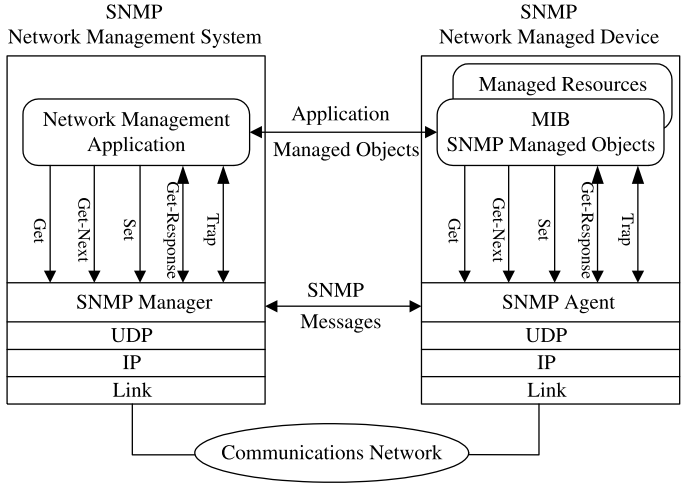
\includegraphics[width=\textwidth,keepaspectratio=true]{snmp_stack}
		\fonte{Adaptado pelo autor de \citetexto{Ding2009}.}
	\end{minipage}
\end{figure}

\begin{figure}
	%TODO Melhorar imagens
    \caption{Estrutura dos Pacotes SNMP}
	\label{fig:snmp-pdu}
    \centering
    \begin{subfigure}[b]{0.60\textwidth}
        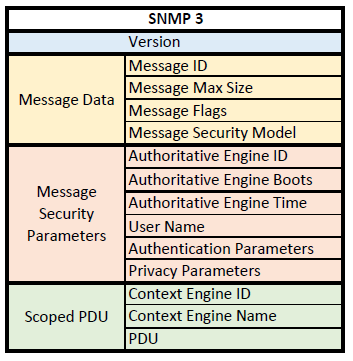
\includegraphics[height=9cm,width=\textwidth,keepaspectratio=true]{snmp_pdu_v3}
		%\fonte{muito texto longo longo longo}
    \end{subfigure}
\hfill
    \begin{subfigure}[b]{0.30\textwidth}
        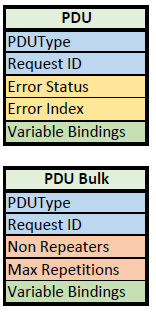
\includegraphics[height=9cm,width=\textwidth,keepaspectratio=true]{snmp_pdu}
		%\fonte{muito texto longo longo longo}
    \end{subfigure}
\\
    \begin{subfigure}[b]{0.27\textwidth}
        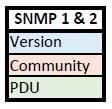
\includegraphics[height=4cm,width=\textwidth,keepaspectratio=true]{snmp_pdu_v1}
		%\fonte{muito texto longo longo longo}
    \end{subfigure}
\hspace{.1\textwidth}
    \begin{subfigure}[b]{0.27\textwidth}
        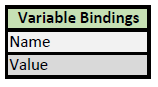
\includegraphics[width=\textwidth,keepaspectratio=true]{snmp_pdu_varbinds}
		%\fonte{muito texto longo longo longo}
    \end{subfigure}
\fonte{Adaptado pelo autor com base em 
	\citetexto{perkins1997understanding}, 
	\citetexto{Stallings1998}, 
	\citetexto{stallings1999snmp} e
	\citetexto{Mauro2009}.
}
\end{figure}


Projetado desde o princípio para ser o protocolo de gerência de redes 
associado aos protocolos de internet (TCP/IP), o SNMP trabalha nativamente 
sobre o serviço de datagramas UDP (\textit{User Datagram Protocol}).
Ao contrário do TCP, que exige o estabelecimento de uma conexão antes de 
comunicar-se, o UDP evita este custo enquanto não garante a entrega nem 
a ordenação das mensagens.
Apesar dessas deficiências, os ganhos obtidos são suficientes para justificar 
sua escolha pois um vez que os metadados do pacote são menores, seu uso reduz 
o impacto na operação normal da rede e aumenta as chances de sucesso na 
comunicação em redes sobrecarregadas \cite{Mauro2009}.


Entretanto a situação torna-se mais delicada quando \textit{traps} são 
consideradas. 
A ausência de confirmação por parte do UDP faz com que não seja possível ao 
emissor saber se sua mensagem chegou ao destino e, no caso das \textit{traps}, 
pode significar a perda de um evento importante \cite{Clemm2006}.
Para casos onde é estritamente necessária a confirmação de um evento, foi 
adicionada a operação \textit{inform} que realiza este controle através da 
aplicação ao invés do protocolo de transporte.


Apesar de projetado para o funcionamento sobre redes TCP/IP, o SNMP, devido ao 
seu sucesso, ganhou compatibilidade com outras plataformas como AppleTalk e 
IPX, além de projetos para interoperabilidade com o modelo ISO 
assim que ele entrasse em uso \cite{Hunt1997}.
Entretanto tais tecnologias perderam espaço e hoje não têm mais relevância nas 
redes de computadores e tampouco na sua gerência.
Para comunicação sobre UDP, o SNMP utiliza a porta 161 para todas operações 
exceto \textit{traps} e \textit{informs}, quando usa a porta 162 
\cite{Mauro2009}.


Ao longo de sua evolução o SNMP passou por revisões na estrutura de suas 
mensagens, com a principal delas ocorrendo na transição entre as versões 1 e 2.
Tais correções tiveram por objetivo unificar a arquitetura e 
simplificar o seu tratamento tanto no agente quanto no gerente 
\cite{perkins1997understanding}.
Apesar das alterações no formato das mensagens, a arquitetura do modelo SNMP, 
como ilustrada pela ~\autoref{fig:snmp-stack}, não foi alterada, 
seguindo estável desde seu projeto.


Com a padronização de sua terceira versão o SNMP passou a contar com 
funcionalidades maduras de segurança, entretanto esta evolução trouxe 
consigo um significativo aumento na complexidade do protocolo
\cite{Mauro2009}.
Este crescimento fica evidente quando inspeciona-se a estrutura de um pacote 
SNMP das versões 1 e 2 comparado com a versão 3.
Com a ajuda da \autoref{fig:snmp-pdu}, percebe-se que as funcionalidades de 
segurança incorrem um custo tanto no tamanho dos pacotes quanto na 
simplicidade do protocolo.


Apesar da mudança no pacote SNMP, a estrutura da PDU (\textit{Protocol Data 
Unit}, ou, em tradução livre, Unidade de Dados do Protocolo) manteve-se 
estável.
A PDU é responsável por encapsular os dados de requisições e respostas 
realizadas através do SNMP e, para isso, conta com campos de metadados 
e dados \cite{perkins1997understanding}.


Todas as operações disponibilizadas pelo SNMP compartilham a mesma PDU, 
com ressalvas no caso do \textit{get-bulk}, sendo esta uma prova concreta
da simplicidade do SNMP, uma vez que a estrutura compartilhada facilita
a implementação de agentes \cite{Clemm2006}
Na \autoref{tab:pdu-operacao} é detalhado o significado de cada um dos
campos da PDU conforme a operação realizada.
Cabe destacar que os campos \textit{error status} e \textit{error index} 
adquirem outro significado quando usados na requisição \textit{get-bulk},
informando quais dos itens nos \textit{variable bindings} devem ser 
interpretados como repetidos ou não \cite{perkins1997understanding}.


Cabe, também, atenção especial aos \textit{variable bindings}, que indicam 
os objetos de interesse da requisição e da resposta.
Neste campo espera-se uma lista contendo os nomes (identificadores na MIB) 
e os valores dos campos sobre os quais o gerente deseja operar 
\cite{Simoneau1999}.
No caso de respostas, \textit{sets} e \textit{traps} 
(considerando também \textit{informs} e \textit{reports})
estarão presentes os valores que definem os objetos, enquanto nas requisições
devem conter um indicador de campo vazio (NULL) \cite{Clemm2006}.
Nessa estrutura reside a capacidade do SNMP de obter e definir diversas 
informações de gerência em uma única requisição e de maneira atômica.


% Maldito seja o momento em 
% que decidi fazer uma tabela
\afterpage{%
    \clearpage			% Flush earlier floats (otherwise order might not be correct)
    \begin{landscape}	% Landscape page
        \centering
		\begin{table}
			\caption{Relação dos campos da PDU e seu uso de acordo com a operação}
			\label{tab:pdu-operacao}
			\renewcommand{\arraystretch}{1.5}%
		    \begin{tabulary}{\textwidth}{
|p{2.5cm}	% campos
|p{3.75cm}	% response
|p{3.0cm}	% set
|p{1.25cm}	% trap
|p{1.25cm}	% inform
|p{1.25cm}	% report
|p{3.75cm}	% get
|p{1.5cm}	% get-next
|p{3.75cm}	% get-bulk
|}
\hline
  ~ 
& \textbf{\textit{response}} 
& \textbf{\textit{set}} 
& \textbf{\textit{trap}} 
& \textbf{\textit{inform}} 
& \textbf{\textit{report}} 
& \textbf{\textit{get}} 
& \textbf{\textit{get-next}} 
& \textbf{\textit{get-bulk}} 
\\ 
\hline
  PDU Type 
& 0xA2 
& 0xA3 
& 0xA7 
& 0xA6 
& 0xA8 
& 0xA0 
& 0xA1 
& 0xA5 
\\
\hline
  Request ID 
& Copia o valor da requisição 
& \multicolumn{7}{c|}{Número gerado pelo solicitante para identificar a requisição} 
\\
\hline
  Error Status / \newline 
  Non Repeaters 
& Indica o código do erro ocorrido no processamento da resposta 
& \multicolumn{6}{c|}{Não utilizado, deve ser enviado zerado} 
& Assume o papel de Non Repeaters, indicando quantos dos itens presentes nos Variable Bindings devem retornar apenas uma ocorrência 
\\
\hline
  Error Index / \newline 
  Max Repetitions 
& Indica a posição do item nos Variable Bindings que causou o erro 
& \multicolumn{6}{c|}{Não utilizado, deve ser enviado zerado} 
& Assume o papel de Max Repetitions, indicando quantas vezes deve obter os itens restantes nos Variable Bindings 
\\
\hline
  Variable \newline 
  Bindings 
& Lista de Nomes e Valores conforme recebido na requisição porém com os valores preenchidos com os dados atuais do dispositivo 
& Lista de Nomes e Valores contendo os valores que deseja-se definir para os objetos no dispositivo destino 
& \multicolumn{3}{p{4.6cm}|}{Lista de Nomes e Valores contendo os dados relevantes à notificação e obrigatoriamente informando o uptime do dispositivo e o tipo de notificação} 
& Lista de Nomes e Valores contendo os identificadores dos objetos aos quais deseja-se obter o valor e com o valor na requisição definido como NULL 
& \multicolumn{2}{p{5.75cm}|}{Lista de Nomes e Valores contendo os identificadores parciais dos objetos aos quais deseja-se obter o valor e com o valor na requisição definido como NULL} 
\\ 
\hline
    		\end{tabulary}
			\fonte{Adaptado pelo autor com base em 
				\citetexto{perkins1997understanding} e 
				\citetexto{stallings1999snmp}.
			}
		\end{table}
    \end{landscape}
	\clearpage
}


\section{MIB}

Parte integral da gerência de redes é a definição de um idioma comum que será 
usado entre gerentes e agentes. O protocolo, seja SNMP ou qualquer outro, faz 
parte da solução mas sozinho não é capaz de preencher todos os requisitos 
necessários para o estabelecimento de uma linguagem compreendida por todos os 
interessados na gerência e, apesar de especificar o formato das mensagens, o 
protocolo não determina como as informações serão representadas.
Esta é a função da Base de Informações de Gerência 
(em inglês \textit{Management Information Base}, MIB).

O papel da MIB é especificar a organização lógica e quais são os dados 
disponíveis para que aplicações se comuniquem de maneira padronizada 
\cite{Silva2005}.
Sua importância deve-se ao fato de ser 
``uma definição precisa das informações acessíveis através de um protocolo de 
gerência de redes''
\cite[p.~152]{Leinwand1996} 
e de que as
``informações de gerência estão no cerne da comunicação que ocorre entre 
gerentes e agentes''
% Management information is at the core of management communication that 
% takes place between managers and agents
\cite[p.~227]{Clemm2006}.

Sua origem ``deriva do modelo OSI/ISO de gerência de redes''
% stems from the OSI/ISO Network management model
\cite[p.~46]{Ding2009} 
e indica que
``como um conceito, uma MIB não depende de nenhum protocolo de gerência''
% as a concept, a MIB does not depend on any particular management protocol
\cite[p.~222]{Clemm2006}.
Porém este nem sempre é o caso e, como o próprio \citetexto{Clemm2006} 
explica, 
``apesar de, em teoria, MIBs poderem ser definidas de forma verdadeiramente 
independente do seu protocolo, na prática diferentes protocolos exigem sua 
própria maneira''
% Although in theory MIBs could be defined to be truly independent of the 
% management protocol, in practice, different management protocols require 
% their own specific way. [p 201 / 179]
.
Este foi o caso do SNMP e do modelo ISO, onde inicialmente previa-se que ambos 
compartilhariam as mesmas MIBs, porém diferenças nos protocolos forçaram o 
desenvolvimento independente \cite{Hunt1997,stallings1999snmp,Leinwand1996}.

Estruturada como uma árvore, a MIB abriga e define todas as informações de 
gerência para determinado dispositivo ou classe de dispositivos, ou seja, 
``MIBs são especificações contendo as definições das informações de 
gerenciamento para que sistemas em rede possam ser monitorados, configurados e 
controlados''
% MIBs are specifications containing definitions of management information so 
% that networked systems can be remotely monitored, configured, and controlled.
\cite[p.~1]{perkins1997understanding}.
Outra forma de visualizar a MIB é como uma coleção de objetos em um banco de 
dados virtual usado para gerir entidades de rede, tais como computadores, 
roteadores e impressoras 
% It comprises a collection of objects in a (virtual) database used 
% to manage entities (such as routers and switches) in a network 
% [p 46 / 67]
\cite{Ding2009}, permitindo representar uma visão lógica do dispositivo sendo 
gerenciado e criando uma camada de abstração especificamente para fins de 
gerência de redes 
% it represents an abstraction and a view of the 
% device being managed for management purposes
\cite{Clemm2006}.
Desta forma 
``qualquer tipo de informação estatística ou de estado que pode ser acessada 
pelo gerente está definida na MIB''
% Any sort of status or statistical information that 
% can be accessed by the NMS is defined in a MIB
\cite[p.~4]{Mauro2009}.

É importante notar que um agente pode, e é encorajado a, 
implementar mais de uma MIB concorrentemente 
% multiple MIBs might be supported concurrently by the same managed device, 
% each by its own management agent
\cite{Clemm2006}, 
isto é possível pois 
``permite-se a indivíduos e fornecedores definir MIBs para seu próprio uso'' 
% vendors, and individuals, are allowed to define MIB 
% variables for their own use
\cite[p.~5]{Mauro2009}. 
Grandes fabricantes como Cisco e 3Com (agora HP), além de suportar um 
conjunto básico de MIBs, fornecem, juntamente com seus equipamentos, MIBs 
próprias e específicas para determinados produtos.
Desta forma podemos concluir que uma MIB 
``pode ser pensada como a especificação que define os objetos gerenciados que 
um dispositivo ou fornecedor suporta''
% The MIB can be thought of as a specification that defines 
% the managed objects a vendor or device supports
\cite[p.~27]{Mauro2009}.


\chapter{Internet das Coisas}

A Internet das Coisas pode ser caracterizada como um paradigma no qual uma 
infinidade de dispositivos, embarcados em objetos cotidianos, podem coletar 
dados sobre seu ambiente e, através de esquemas de endereçamento, comunicar-se 
entre si em busca de um objetivo comum \cite{Atzori2010b}.
Indústria e academia estão cientes das possibilidades que este modelo 
apresenta e cooperam em prol do alcance desta visão através de parcerias e 
trocas de experiência  \cite{ITU2005}.
Apesar dos esforços, a tecnologia atual não permite, de maneira economicamente 
viável, alcançar as proporções necessárias para a criação de uma verdadeira 
Internet das Coisas, tornando os experimentos não mais do que protótipos de 
escala reduzida \cite{Smith2012}.


Neste capítulo são apresentados os principais conceitos que possibilitaram a 
concepção da ideia de uma Internet das Coisas e sua definição conforme 
interpretada neste trabalho.
Ainda é abordada aqui a importância da IoT para revolucionar a maneira como a 
sociedade adquire informações e conhecimento sobre si mesma, transformando-os 
em sabedoria, assim como os principais desafios e oportunidades ligados à 
realização deste paradigma.


\section{Origem}

	Diversas tecnologias contribuíram com os avanços necessários para o 
	desenvolvimento da Internet das Coisas. A partir dos estudos em áreas como 
	etiquetas de Identificação por Radiofrequência (RFID), Redes de 
	Sensores sem Fio (WSN), Protocolo de Internet versão 6 (IPv6) e Smart 
	Objects foi possível atingir o atual nível de maturidade da IoT.
	Abaixo são apresentadas as principais tecnologias nas quais o conceito de 
	Internet das Coisas se apóia e que possibilitaram o seu desenvolvimento.

% Citar \cite[p.~8]{Buckley2006} sobre os graus de sofisticação dos 
%dispositivos

%	Originado a partir das pesquisas aplicadas de etiquetas de Identificação 
%	por radiofrequencia (RFID) \cite{Welbourne2009}, o conceito de Internet 
%	das Coisas foi sendo moldado de acordo com os avanços tecnológicos obtidos 
%	nos campos relacionados. 

\subsection{RFID}
	Etiquetas RFID representam uma nova geração dos mecanismos de 
	identificação de objetos \cite{Brock2001}. Diferentemente dos códigos de 
	barras, as \textit{tags} RFID utilizam comunicação via radiofrequência, o 
	que, segundo \citetexto{Want2006}, possibilita uma maior distância de 
	leitura e, adicionalmente, elimina a necessidade de visada direta. O autor 
	afirma ainda que é possível que as etiquetas contenham memória de leitura 
	e escrita, permitindo descrever estados do objeto identificado, além de 
	sensores que podem indicar informações sobre o item (se ele sofreu quedas 
	ou se permaneceu dentre os limites de temperatura, por exemplo).
	
	Iniciativas preliminares no campo da Internet das Coisas contemplaram 
	principalmente o uso de RFIDs para realizar o rastreamento de objetos em 
	um ambiente dotado de diversos leitores RFID ou para ativar determinados 
	comportamentos em um sistema computacional de acordo com dados obtidos 
	através da leitura de uma etiqueta. Os trabalhos de \citetexto{Want1999}, 
	\citetexto{Floerkemeier2007a} e \citetexto{Welbourne2009} apresentam 
	implementações concretas utilizando-se de RFIDs.

\subsection{WSN}
	Diferentemente das \textit{tags} RFID, que não realizam processamento e 
	são geralmente passivas \cite{Atzori2010b}, as Redes de Sensores sem Fio 
	são compostas de pequenos dispositivos que, apesar da capacidade reduzida, 
	efetuam coleta e processamento de dados \cite{Sakthidharan2012}. Segundo 
	\citetexto{Sung2007}, boa parte das aplicações de WSNs são voltadas para 
	o monitoramento de ambientes físicos, contemplando fins militares, 
	ecológicos e industriais \cite{Suhonen2012}. Pesquisas relacionando RFID e 
	WSNs, em direção a uma visão de Internet das Coisas, foram realizadas por 
	\citetexto{Sung2007}, \citetexto{Zhang2011a} e \citetexto{Hada2011}, 
	comprovando a viabilidade da proposta.
	
	De acordo com \citetexto{Liu2012}, a capacidade de coletar e processar 
	dados de maneira autônoma é uma das fundações da IoT, tornando as WSNs uma 
	das áreas de pesquisa que mais contribuíram para o seu desenvolvimento. 
	\citetexto{Perera2013} corrobora ao afirmar que a IoT não pode existir sem 
	o apoio das WSNs, pois elas fornecem a maior parte da infraestrutura de 
	hardware para a comunicação e coleta de informações contextuais.

\subsection{Gateway IoT}
	Apesar do sucesso das WSNs para a comunicação em curta distância, 
	\citetexto{Zhu2010} afirma que existe dificuldade 
	em conectar redes de sensores à internet devido a falta de padronização 
	nos protocolos de comunicação. Para superar esta dificuldade foi 
	estabelecido o conceito de dispositivo coordenador, também chamado de 
	\textit{gateway} \cite{Steenkamp2009}. 
	Assim como as WSNs, os protótipos iniciais de IoT conectavam-se à internet 
	através do coordenador, um dispositivo mais potente que faz o papel de 
	roteador na rede \cite{Kuryla2010} e, por não apresentar as mesmas 
	restrições dos sensores, é encarregado de prover 
	conectividade externa (através de 
	tecnologias como GSM, CDMA e WLAN, por exemplo) \cite{Liu2012}.
	
	As implementações de \citetexto{Zhu2010}, \citetexto{Steenkamp2009} e 
	\citetexto{Hada2011} apresentam resultados e percepções sobre o uso de 
	\textit{gateways} entre WSNs e a internet, viabilizando a criação de 
	aplicações que demonstram, na prática, o conceito de Internet das Coisas.

\subsection{IPv6}
	Uma vez cumprido o objetivo de conectar as WSNs a internet o próximo passo 
	consiste em propiciar conectividade a cada dispositivo individualmente 
	\cite[p.~13]{Atzori2010b}, efetivamente tornando-o parte da internet.
	Para tanto, a escolha considerada mais sábia por \citetexto{Mattern2010a} 
	é de utilizar-se dos mesmos protocolos já estabelecidos pela internet, 
	favorecendo a interoperabilidade.
	Sobre o uso de endereços IP como forma de 
	identificação \citetexto{Sundmaeker2010} dizem que:
	\begin{quote}
		a ideia de atribuí-los a cada um dos aproximadamente 5 
		mil objetos diários que nos cercam, é bastante atraente.
		Com a tecnologia certa em cada objeto (uma etiqueta RFID, por exemplo) 
		e a rede certa nos arredores, será fácil localizar e catalogar itens 
		em poucos segundos e colher os benefícios da vasta quantidade de novas 
		informações que a comunicação entre eles vai prover. IPv6 é 
		indiscutivelmente um dos passos para tornar a Internet das Coisas uma 
		realidade.
		\cite[p.~15]{Sundmaeker2010}.
	\end{quote}
	
	Orientadas por esta visão, companhias como Intel, Cisco e SAP formaram em 
	2008 a aliança ``IP para Objetos Inteligentes'' (IPSO), reforçando o 
	interesse da indústria pela conectividade direta entre dispositivos 
	\cite{Dunkels2008, Mattern2010a}. 
	Aliada a esse interesse, a Força Tarefa de Engenharia da Internet, IETF, 
	vem desenvolvendo o protocolo IPv6 sobre Rede Local Pessoal Sem Fio de 
	Baixo Consumo, 6LoWPAN, que define os mecanismos para troca de mensagens 
	IPv6 sobre redes IEEE 802.15.4, especialmente projetada para o caso da 
	Internet das Coisas \cite{Gomez2010}.

\subsection{Smart Objects}
	Contrastando com as etiquetas RFID, o conceito de Objetos Inteligentes 
	(\textit{Smart Objects}) compreende objetos físicos/digitais autônomos 
	aumentados com capacidades sensoriais, de processamento e rede 
	\cite{Gellersen2001}.
	Estes objetos foram classificados, no trabalho de \citetexto{Kortuem2010a}, em 
	três grandes grupos de acordo com seu grau de percepção e, 
	consequentemente, complexidade. Sendo eles: consciência à nível de 
	atividade, de política e de processo.
	Segundo \citetexto{Dunkels2008}, a adoção e popularização dos Objetos 
	Inteligentes tem sido dificultada pela grande quantidade de sistemas 
	fechados e proprietários, o que dificulta, ou até mesmo impossibilita, a 
	integração entre soluções. 
	
	Espera-se que as principais habilidades de um Objeto Inteligente digam 
	respeito ao compartilhamento de informações (entre dispositivos e 
	usuários) e a consciência do contexto em que estão inseridos 
	\cite{Gellersen2001}. 
	Os autores ainda enfatizam que tais objetos ``serão deliberadamente 
	limitados em sua capacidade computacional, memória e poder de 
	processamento a níveis adequados para um propósito específico''. 
	Seguindo esta tendência, \citetexto{Mattern2010a} prevêem que a tecnologia 
	caminha em direção a um modelo onde Objetos Inteligentes efetivamente se 
	comuniquem entre eles mesmos, serviços na internet e seus usuários.
	
	Experiências no planejamento e execução de aplicações compostas por 
	\textit{Smart Objects} podem ser encontradas nos trabalhos de 
	\citetexto{Gellersen2001}, \citetexto{Gellersen2004}, 
	\citetexto{Holmquist2004}, através do projeto Smart-Its, e 
	\citetexto{Kortuem2010a}, abordando questões de saúde e segurança, gestão 
	de processos e modelos de negócio por intermédio de um único dispositivo 
	aplicado ao ramo da construção civíl.

\section{Definição}

	Diversas são as definições disponíveis para o termo Internet das 
	Coisas (IoT). \citetexto{Atzori2010b} atribuem a grande variedade de 
	definições às diferentes visões que cada organização, dependendo dos 
	seus objetivos, tem, geralmente sendo orientadas a internet ou as 
	coisas. Apesar das diferenças o conceito de IoT é, para 
	\citetexto{Coetzee2011}:
	
	\begin{quote}
		uma visão onde objetos se tornam parte da internet: onde cada 
		objeto é unicamente identificável e acessível à rede, sua posição 
		e status conhecidos, onde serviços e inteligência são acrescidos a 
		esta internet expandida, fundindo o mundo físico e o digital~
		\cite{Coetzee2011}.
	\end{quote}
	
	Segundo \citetexto{Sundmaeker2010}, dentre as mais citadas estão as 
	definições por Kevin \citetexto{Ashton2009} e David 
	\citetexto{Brock2001} do Auto-ID Labs e da União Internacional de 
	Telecomunicações, \citetexto{ITU2005}. Enquanto a primeira é focada na 
	identificação e detecção de objetos através do uso de RFIDs, a segunda 
	aborda uma definição mais ampla, detalhada a seguir.
	
	Em sua definição, a \citetexto{ITU2005} sugere que a Internet das 
	Coisas, através de suas tecnologias, será capaz de conectar objetos de 
	maneira inteligente e sensorial, combinando avanços nos campos de:
	\begin{itemize}
		\item Identificação --- \textit{Tagging things}: Tecnologias para 
		reconhecimento e rastreamento de objetos, baseadas principalmente 
		em RFID. Possibilitam uma forma primitiva de integração entre o 
		real e o virtual;
		
		\item Sensores --- \textit{Feeling things}: Tecnologias 
		relacionadas a WSNs, utilizando-se dos conhecimentos já adquiridos 
		pelas pesquisas nesta área. Sensores ampliam a quantidade de 
		informações contextuais para aplicações, possibilitando um melhor 
		mapeamento do seu ambiente por meio de parâmetros como: 
		temperatura, luminosidade, vibração, nível de ruído, entre outros;
		
		\item Sistemas embarcados --- \textit{Thinking things}: Refere-se 
		a crescente capacidade de embutir microcontroladores e 	
		processadores em objetos da vida cotidiana, efetivamente 
		possibilitando a criação de objetos inteligentes. Com a redução de 
		custo e tamanho, a substituição de circuitos de propósito 
		específico por processadores multipropósito é favorecida, criando 
		uma nova geração de objetos;
		
		\item Nanotecnologia --- \textit{Shrinking things}: Abordando o 
		impacto e as possibilidades do uso altamente difundido de 
		tecnologias de nano escala. Dentre as previsões estão circuitos 
		menores, mais econômicos e baratos, além do uso de novos 
		materiais, como grafeno e nanotubos, na fabricação destes 
		dispositivos.
	\end{itemize}
	
	Entretanto, a riqueza de possibilidades abertas pela IoT pode ser 
	explicada simplesmente pela análise individual de seus termos 
	constituintes, ou seja, a combinação de internet e coisas. Segundo 
	\citetexto{Simpson2005}, no Oxford English Dictionary, a internet é 
	``uma rede global de computadores provendo diversos serviços de 
	informação e comunicação, constituída de redes interconectadas usando 
	protocolos padronizados de comunicação''.
	
	Coisas, por outro lado, não tem uma definição precisa, podendo variar 
	conforme o contexto e o foco da aplicação. \citetexto{Coetzee2011} 
	apresentam uma definição abrangente direcionada para IoT:
	
	\begin{quote}
		A definição de ``coisas'' na visão da IoT é muito ampla e inclui 
		uma variedade de elementos físicos. Estes incluem objetos pessoais 
		que carregamos como \textit{smart phones}, \textit{tablets} e 
		câmeras digitais. Ela também inclui elementos em nosso ambiente 
		(seja em casa, no carro ou no trabalho) assim como coisas 
		equipadas com \textit{tags} (RFID ou outras) que se tornam 
		conectadas através de um portal de acesso (um \textit{smart 
			phone}, por exemplo).~
		\cite{Coetzee2011}.
	\end{quote}
	
	Identifica-se uma mudança gradual na definição do conceito de Internet 
	das Coisas, inicialmente contemplando apenas mecanismos de 
	identificação e, impulsionado pela evolução tecnológica, passando a 
	versar sobre dispositivos inteligentes e diretamente conectados à 
	internet sem a necessidade de intermediários. Segundo 
	\citetexto{Buckley2006} a transformação no conceito de IoT é resultado 
	tanto de avanços tecnológicos quanto de interesse mercadológico 
	impulsionado pelos potenciais benefícios.

% Based on the above view of “things” an enormous number of devices and things 
% will be connected to the Internet, each providing data and information and 
% some, even services.

\section{Importância}

	Uma vez estabelecida a definição de Internet das Coisas, é possível 
	compreender o impacto social e tecnológico deste conceito. A internet 
	causou uma revolução na maneira com que compartilhamos informação e 
	conhecimento, gerando, de acordo com \citetexto{Carr2010}, mudanças 
	até mesmo em nossa estrutura cerebral.
	
	Classificada como a terceira onda da computação \cite{Register2013}, 
	os conceitos de IoT poderão ser aplicados a diversos setores 
	produtivos, desde a indústria ao setor público. Os possíveis 
	benefícios obtidos através de uma vasta rede de dispositivos 
	interconectados fez com que especialistas como \citetexto{Hung2012}, 
	da Gartner, classificassem a IoT como um paradigma transformacional.
	
	\citetexto{Cisco2011} ressaltam que a importância da IoT está 
	profundamente interligada com a maneira como a humanidade se desenvolveu: 
	``Humanos evoluem porque se comunicam. Assim que o fogo foi descoberto 
	e compartilhado, por exemplo, ele não precisou ser redescoberto, 
	apenas comunicado''. Ainda sob este ponto de vista afirma que, com a 
	aplicação dos conceitos de IoT, haverá um aumento exponencial na 
	quantidade de dados disponível:
	
	\begin{quote}
		considere que a IoT representa a próxima evolução da internet, 
		levando a um enorme salto na sua habilidade de coletar, analisar e 
		distribuir dados que podemos transformar em informação, 
		conhecimento e, finalmente, sabedoria.~
		\cite[p.~2]{Cisco2011}.
	\end{quote}

	\begin{figure}
		\caption{Hierarquia do conhecimento}
		\label{fig:wkid}
		\centering
		\begin{minipage}{.8\textwidth}
			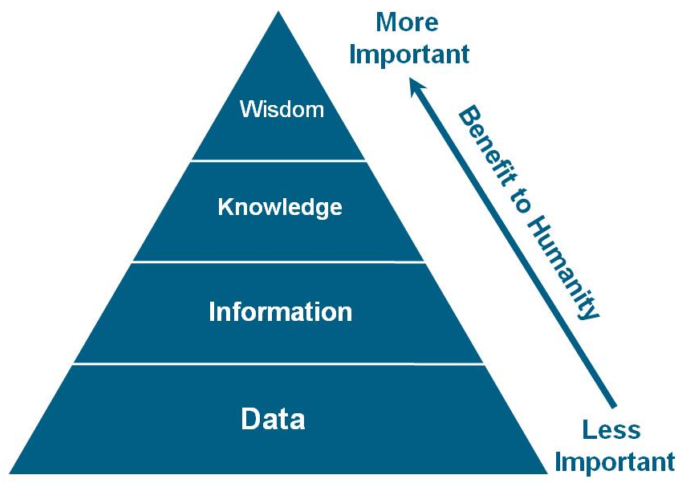
\includegraphics[width=\textwidth]{wkid}
			\fonte{\citetexto{Cisco2011}}
		\end{minipage}
	\end{figure}


\section{Desafios}


A realização de uma visão de Internet das Coisas não ocorrerá sem desafios, 
tanto sociais e políticos quanto tecnológicos.
As implicações ligadas a existência de uma infinidade de dispositivos 
coletando e transmitindo informações sobre a vida cotidiana de seus usuários 
já causa grandes preocupações entre membros da indústria e da academia.
Desenvolvimentos tecnológicos, necessários para viabilizar a difusão do 
conceito de IoT, também representam grandes barreiras no avanço deste 
paradigma.


\begin{figure}
	\caption{Estratégias para proteção de privacidade}
	\label{fig:iot-privacy}
	\centering
	\begin{minipage}{.8\textwidth}
		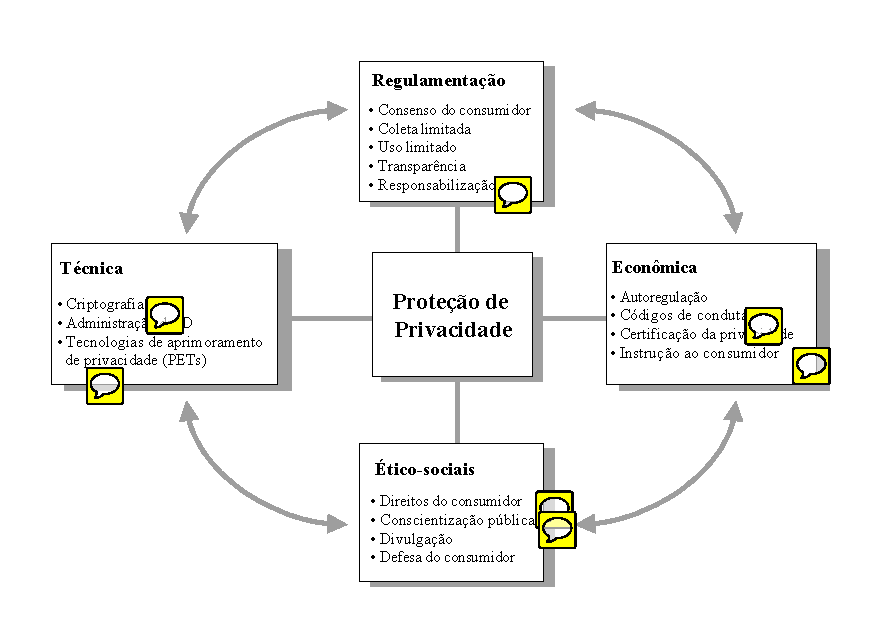
\includegraphics[width=\textwidth,keepaspectratio=true]{ITU_privacy[107]}
		\fonte{Adaptado pelo autor de \citetexto{ITU2005}.}
	\end{minipage}
\end{figure}


No âmbito social, as dificuldades em tornar real a visão da Internet das 
Coisas concentram-se principalmente em torno da privacidade.
Diversos autores demonstram receio quanto a maneira com que os dados obtidos 
serão utilizados, havendo, inclusive, propostas de códigos de conduta 
específicos para este paradigma \cite{ITU2005}.
Existe a noção de que há um balanço a ser atingido através dessas tecnologias, 
de um lado a proteção à privacidade, e de outro o conforto obtido através do 
uso destas informações \cite{Atzori2010b}.


Assim como a revolução industrial causou um aumento na dependência da 
civilização na energia elétrica, \citetexto{Mattern2010a} ponderam que a 
implantação de uma Internet das Coisas a nível global trará um aumento na 
dependência de conectividade.
Há de se convir que atualmente já percebe-se um aumento na dependência por 
computadores e conectividade, como nota \citetexto{Carr2010}, contudo o 
aumento explosivo na quantidade de dispositivos, previsto por 
\citetexto{Cisco2011} para a casa de 50 bilhões em 2020, vai agravar ainda 
mais a situação.


O medo de viver em uma era Orwelliana\footnote{
	George Orwell era um escritor inglês que, em seu livro 1984, caracterizou 
	um ditador totalitário que vigiava a todos através de câmeras e 
	denominava-se Big Brother.
}, com vigilância integral sobre o indivíduo, torna-se uma possibilidade real 
e factível.
Desta forma, há grandes receios por parte da comunidade acadêmica sobre a 
forma com que tais dados serão utilizados e, conforme aponta a 
\autoref{fig:iot-privacy}, como serão protegidos. 
A respeito da privacidade, \citetexto{Buckley2006} argumenta que dentre as 
principais questões em aberto neste contexto encontram-se: a propriedade dos 
dados, quem é o dono dos dados coletados; a gestão de acessos, quem pode 
acessar e qual é o nível de acesso aos dados; a autorização para transmissão, 
quem está ciente e/ou autoriza a transmissão dos dados para terceiros; e a 
neutralização de objetos, como desabilitá-los de forma permanente.


Relacionada a privacidade, existem ainda questões de segurança que previnem a 
difusão da Internet das Coisas.
Dada a reduzida capacidade de processamento dos dispositivos que integram o 
paradigma da IoT, técnicas de criptografia e segurança de dados acabam sendo 
de aplicabilidade limitada, portanto ainda são necessários desenvolvimentos 
nestas técnicas \cite{Sundmaeker2010}.
Mecanismos de identificação, como chaves pública-privadas, por exemplo, devem 
também ser melhorados e padronizados para o uso no contexto de IoT, uma vez 
que serão responsáveis por manter o controle e permissionamento necessário 
para o acesso aos dados contidos nos dispositivos, assim como mecanismos para 
revogação destas identificações \cite{Buckley2006}.
Ainda permeando a segurança está a preocupação com a clonagem de \textit{tags} 
e dispositivos, algo que pode comprometer toda uma rede assim como colocar em 
risco a segurança de outras pessoas, como no caso de um passaporte clonado 
\cite{ITU2005}. 


A quantidade de dados gerados através dos dispositivos que compõem a Internet 
das Coisas também apresenta seus próprios desafios. 
\citetexto{Coetzee2011} define este fenômeno como ``dilúvio de dados'', onde 
deve-se provisionar desde espaço de armazenamento até capacidade de rede para 
tratar do volume de informação. Existe, ainda, o problema de como interpretar 
todos estes novos dados que, devido ao seu volume, nem sempre fazem sentido 
com técnicas simples de análise \cite{ITU2005}.
Apesar de diretamente relacionado às questões de segurança e privacidade, o 
problema da quantidade de informação gerada permeia também questões técnicas.


Os desafios de âmbito técnico apresentados pelo paradigma da Internet das 
Coisas são muitos e diversos, caracterizando, em alguns casos, uma área de 
estudo própria. Portanto são apresentados na lista abaixo uma compilação dos 
desafios técnicos conforme definidos por 
\citetexto{ITU2005}, 
\citetexto{Buckley2006}, 
\citetexto{Mattern2010a} e 
\citetexto{Sundmaeker2010}:

\begin{itemize}
	
	\item \textbf{Energia:}
Melhorias na capacidade de baterias e nas técnicas de conversão de energia a 
partir de outras fontes (como vibração, luz e calor) são necessárias para 
aumentar a utilidade dos dispositivos, uma vez que a limitação energética faz 
com que outras características do aparelho também tenham que ser limitadas;
	
	\item \textbf{Antenas:}
Visando aumentar o alcance das comunicações e a duração das baterias, 
desenvolvimentos em técnicas de processamento de sinais e no projeto de 
antenas também são desejáveis para dispositivos da IoT;
	
	\item \textbf{Protocolos:}
Reduções no custo das comunicações e métodos de tolerância a falhas são 
necessários para tornar a comunicação sem fio mais confiável, tendo como 
efeito colateral uma redução no gasto energético (uma vez que mensagens não 
precisarão ser retransmitidas);
	
	\item \textbf{Sensores:}
Melhorias na precisão e redução no consumo energético de sensores são, também, 
áreas onde deseja-se desenvolvimento tecnológico. Dado que geralmente mais de 
um sensor integra um dispositivo da Internet das Coisas e as limitações de 
sensores como GPS em ambientes fechados, a superação destas barreiras 
possibilitaria grandes avanços;
	
	\item \textbf{Atuadores:}
Complementando o trabalho dos sensores, os atuadores são responsáveis por 
efetivamente realizar as ações (a partir das decisões tomadas com base nos 
dados de sensores), portanto o seu desenvolvimento traz melhorias para os 
dispositivos e novas possibilidades de produtos e serviços;
	
	\item \textbf{Endereçamento:}
A identificação de dispositivos, não só através de endereços como o IP, também 
é área de estudo relacionada à IoT. O desenvolvimento de ontologias e maneiras 
de endereçar as ``coisas'' conforme a aplicação em questão são necessárias, 
uma vez que o IP não funciona bem com humanos e não provê características 
sobre o dispositivo identificado;
	
	\item \textbf{Busca:}
Da mesma forma como existem algoritmos de busca para documentos na internet, 
é necessário o desenvolvimento de formas de buscar os dispositivos que compõem 
a Internet das Coisas, possivelmente utilizando-se das diferentes técnicas de 
endereçamento e das características de cada um destes dispositivos.s
	
\end{itemize}




\section{Oportunidades}


Conceitos atuais como Big Data fornecem uma amostra das possibilidades de 
extração de conhecimento a partir de grandes conjuntos de dados. 
Com uma Internet das Coisas funcional é possível aumentar a quantidade e a 
qualidade dos dados obtidos e, consequentemente, melhorar também a 
qualidade e a precisão das análises.
Projetos como Hadoop e SAP Hana já encontram-se em uso em diversas 
organizações e contribuem para a gestão e otimização de processos, 
possibilitando a tomada de decisões em tempo real a partir de dados 
vindos de diversas fontes


A grande quantidade de sensores distribuídos geograficamente poderá também 
desempenhar um papel importante na tomada de decisão, possibilitando também, 
em conjunto com atuadores, a automação de tarefas baseadas em dados de 
sensores.
Tais decisões, por mais simples que pareçam, são necessárias ao longo de toda 
a cadeia produtiva na forma de processos industriais, seja no controle de 
umidade do solo, de temperatura ou de peso.
Apesar de serem possíveis hoje, tais controles terão maior valor de negócio, 
uma vez que a integração na Internet das Coisas possibilita o processamento e 
o compartilhamento dessas decisões com outros dispositivos, potencialmente 
servindo como dados de entrada para os demais processos \cite{ITU2005}.


Grandes corporações também se apropriam do conceito de Internet das Coisas 
para a criação de diversos projetos de controle e automação, seja a nível 
residencial, comercial e industrial, expandindo até mesmo à iniciativas 
globais.
HP, IBM e Microsoft através de seus projetos, respectivamente, CeNSE, Smarter 
Planet e Eye-On-Earth demonstraram seu interesse e investimento em direção à 
realização do conceito de Internet das Coisas \cite{Coetzee2011}.
O projeto CeNSE traz, em sua definição, uma descrição da visão de Internet das 
Coisas que vai ao encontro de autores como \citetexto{Atzori2010b}, 
\citetexto{Smith2012} e \citetexto{Perera2013}:

\begin{quote}
CeNSE consiste de uma rede altamente inteligente de bilhões de sensores de 
nanoescala projetados para sentir, provar, cheirar, ver e ouvir o que está 
acontecendo no mundo. Quando completamente implantados, estes sensores irão 
rapidamente reunir dados e transmití-los a potentes motores computacionais, 
que irão, em tempo real, analisar e agir de acordo com as informações usando 
uma nova geração de serviços e aplicações de negócios \cite{HP2009}.

% HP's Central Nervous System for the Earth (CeNSE), a project of HP Labs, is 
% revolutionizing the way information is gathered, communicated, and analyzed. 
% CeNSE consists of a highly intelligent network of billions of nanoscale 
% sensors designed to feel, taste, smell, see, and hear what is going on in 
% the world. When fully deployed, these sensors will quickly gather data and 
% transmit it to powerful computing engines, which will analyze and act upon 
% the information in real time using a new breed of business applications and 
% web services. 
\end{quote}


Os domínios de aplicação afetados pelo paradigma da Internet das Coisas são 
variados e atingem grande parte da população e da indústria.
A difusão de computadores e sistemas de informação pode ser apontada, em 
parte, como responsável pelo grande alcance das tecnologias de IoT, uma vez 
que tais sistemas podem sempre ser aprimorados.
Na lista abaixo encontra-se uma seleção de domínios\footnote{
Elaborada com base nos dados apresentados por 
\citetexto{ITU2005},
\citetexto{Atzori2010b},
\citetexto{Sundmaeker2010},
\citetexto{Smith2012} e
\citetexto{Perera2013}.
} onde são previstas melhorias pelo uso de conceitos e tecnologias da Internet 
das Coisas.


\begin{itemize}
	
	\item \textbf{Aviação e Aeroespacial:}
identificação de peças falsificadas, monitoramento através de redes de 
sensores (dentro e fora da aeronave), identificação de passagens;
	
	\item \textbf{Automotiva:}
sistemas de monitoramento (pressão dos pneus, temperatura do óleo, etc), 
direção autônoma, comunicação veículo--veículo e veículo--infraestrutura;
	
	\item \textbf{Telecomunicações:}
redes peer-to-peer, NFC, carteira digital;
	
	\item \textbf{Prédios Inteligentes:}
automação residencial (luzes e ar-condicionado, por exemplo), monitoramento de 
consumo, assistência a idosos, compras automatizadas;
	
	\item \textbf{\textit{Smart Grids}:}
medição de energia, monitoramento da rede elétrica,  
	
	\item \textbf{Médica e Saúde:}
monitoramento de pacientes, distribuição de medicamentos, medição e 
monitoramento de parâmetros vitais (pulso, temperatura, pressão), dispositivos 
implantados (marcapassos, por exemplo);
	
	\item \textbf{Farmacêutica:}
rastreamento, identificação de produtos falsificados, monitoramento das 
condições de transporte / armazenamento;
	
	\item \textbf{Varejo, Logística e Gestão da Cadeia de Suprimentos:}
monitoramento de entregas, recebimentos e estoque, detecção de furto, 
rastreamento de produtos;
	
	\item \textbf{Manufatura e Gestão de Ciclo de Vida de Produtos:}
otimização do processo de produção, monitoramento do ciclo de vida, 
localização de itens, reciclagem;
	
	\item \textbf{Óleo e Gás:}
monitoramento de barris e contêineres, identificação de produtos tóxicos, 
monitoramento de maquinário e processos, monitoramento de parâmetros de 
operação;
	
	\item \textbf{Segurança, Proteção:}
vigilância ambiental (chuvas, queimadas, poluição, etc), monitoramento de 
infraestrutura (vazamentos e rachaduras, por exemplo), controle de acesso, 
alertas de catástrofes;
	
	\item \textbf{Monitoramento Ambiental:}
monitoramento de desmatamentos e queimadas, monitoramento da qualidade do ar e 
da água, rastreamento de animais;
	
	\item \textbf{Transporte de Pessoas e Mercadorias:}
Sistemas de pedágio e passagens, identificação e triagem de pessoas e 
mercadorias, controle de tráfego, identificação de bagagens;
	
	\item \textbf{Rastreabilidade de Alimentos:}
rastreamento de matéria prima, reconstrução da cadeia de suprimentos, 
identificação de produtos/lotes contaminados, monitoramento das condições de 
armazenamento e transporte;
	
	\item \textbf{Criação e Agricultura:}
identificação e rastreamento de animais, controle e prevenção de doenças e 
pragas, vacinação, redução de intermediários entre produtor e consumidor;
	
	\item \textbf{Mídia, Entretenimento e Bilhetagem:}
geração autônoma de notícias, interatividade através de etiquetas, cobrança 
automatizada de bilhetes e entradas, propagandas interativas;
	
	\item \textbf{Seguros:}
monitoramentos de parâmetros de operação (em troca de descontos, por exemplo), 
acionamento automático da seguradora, previsão de manutenções e trocas;
	
	\item \textbf{Reciclagem:}
monitoramento de emissão de poluentes, logística reversa, rastreamento de 
itens não descartados corretamente.
	
\end{itemize}



\chapter{Proposta para IoT}


Uma vez apresentado o conceito de Internet das Coisas e conhecidos seus 
desafios e oportunidades, torna-se possível identificar pontos de melhoria.
A grande quantidade de dispositivos previstos no contexto de IoT torna sua 
gerência e configuração uma tarefa não trivial e altamente vulnerável a erros 
humanos.
Apesar das iniciativas em busca de autoconfiguração e gestão automatizada, é 
improvável que tais esforços possibilitem uma gerência livre da intervenção de 
operadores.


Ainda que a autoconfiguração forneça um objetivo de longo prazo, a necessidade 
de configurar e gerenciar dispositivos, mesmo que em situações experimentais e 
de escala reduzida, é um problema que já se enfrenta atualmente.
Desta forma, percebe-se o desejo por um método padronizado para a gerência  
destes dispositivos, principalmente no que diz respeito à configuração, uma 
vez que cada sistema operacional (por vezes específico para o domínio de 
aplicação) apresenta mecanismos próprios de gestão e configuração.


Tais necessidades são deveras semelhantes aquelas encontradas nos anos 1980, 
onde profissionais e acadêmicos passavam por grandes dificuldades na gestão 
de suas infraestruturas, seja na forma de um escritório ou de um laboratório.
Semelhanças existem também no que diz respeito à falta de padronização dos 
dispositivos usados em aplicações para a Internet das Coisas, explicitando 
ainda mais a relação com a gerência de redes clássica e o SNMP.


Os problemas semelhantes, no contexto de Internet das Coisas e de gerência de 
redes, tornam oportuno o reuso de estratégias reconhecidamente eficazes e 
postas à prova ao longo dos anos através do SNMP, que acabou tornando-se 
o protocolo \textit{de facto} e sinônimo de gerência de redes.
Contudo, as peculiaridades características da IoT exigem adaptações e revisões 
das antigas estratégias, de forma que aproveite-se também a oportunidade para 
revisitar partes problemáticas do modelo clássico de gerência de redes.


A união dos conceitos de IoT e gerência de redes traz benefícios pois 
possibilita o reuso de ferramentas, protocolos e estratégias de gestão e, 
mesmo que ainda não sejam as mais eficazes, permite obter boa parte dos ganhos 
provenientes do seu uso.
Ainda é possível citar a aderência ao paradigma FCAPS de gerência de redes 
como um subproduto da mescla proposta entre SNMP e IoT, viabilizando o 
reuso de todo um arcabouço de conhecimento frente aos novos desafios 
apresentados pela Internet das Coisas.


\section{Escopo}

De forma a melhor delimitar os objetivos, necessidades e critérios de 
avaliação, este trabalho tem seu escopo de atuação intencionalmente limitado 
à automação residencial.
Neste contexto estão inseridos processos tais como a coleta de dados, ou seja, 
o monitoramento do ambiente (temperatura, umidade, iluminação), 
seus dispositivo (consumo energético, estado) e 
o controle sobre estes dispositivos (ligar, desligar, alterar a temperatura).


Esforços de automação residencial auxiliam na caminhada rumo à casas e prédios 
inteligentes e que regulam, de forma autônoma, parâmetros ambientais como 
temperatura e iluminação baseados em dados a respeito dos hábitos de seus 
moradores.
Entre os ganhos ocasionados por este tipo de automação é possível citar a 
economia de energia e a consequente redução no impacto ambiental, além do 
aumento nos níveis de conforto e segurança das residencias.


A este contexto pertencem as ideias de casas futuristas, vistas em feiras e 
nas obras de ficção-científica, onde, por exemplo, moradores são recebidos com 
torradas e café prontos ao chegar do trabalho, ou com um banho quente à sua 
espera.
Devido às dificuldades tecnológicas e as incompatibilidades entre padrões e 
fornecedores esta visão manteve-se limitada à experimentos.
Entretanto a Internet das Coisas fornece meios que possibilitam chegar ainda 
mais perto da realização desta visão.


\section{Arquitetura}

[\ldots]


Contudo, dados os recursos limitados dos dispositivos da Internet das Coisas, 
conforme detalhado por \citetexto{ietfCNN2013}, a execução de um agente SNMP 
no dispositivo deixa de ser uma tarefa trivial.
Esforços como os de \citetexto{Choi2009} e \citetexto{Kuryla2010} demonstram 
que embutir um agente SNMP em um dispositivo para Internet das Coisas é 
possível, entretanto a implementação ocupa grande parte dos recursos do 
dispositivo, fazendo com que este seja incapaz de executar aplicações de 
usuário, efetivamente inutilizando-o.
Em contrapartida, os trabalhos de \citetexto{Steenkamp2009} e 
\citetexto{Zhu2010} sugerem o uso de um dispositivo dedicado à prover 
conectividade e interoperabilidade aos nós da rede, um \textit{gateway}.
Este dispositivo deve prover comunicação com a internet e servir como um 
tradutor, possibilitando a comunicação em diferentes protocolos, desta forma 
os dispositivos continuariam com suas aplicações de usuário intactas, 
concentrando o custo da tradução no \textit{gateway}.


\begin{figure}
	%TODO Melhorar imagens
    \caption{Arquiteturas de Integração SNMP--IoT}
	\label{fig:arch}
	\centering
    \begin{subfigure}[b]{0.3\textwidth}
        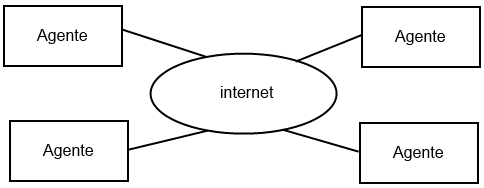
\includegraphics[width=\textwidth,keepaspectratio=true]{arch_snmp}
		\caption{SNMP no dispositivo}
    \end{subfigure}
\hspace{.2\textwidth}
    \begin{subfigure}[b]{0.3\textwidth}
        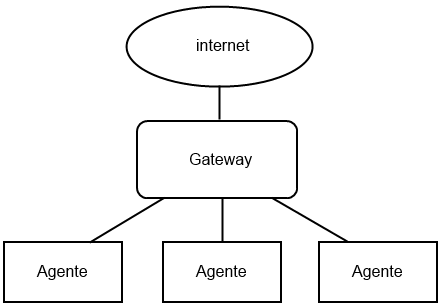
\includegraphics[width=\textwidth,keepaspectratio=true]{arch_gateway}
		\caption{Gateway}
    \end{subfigure}
%TODO verificar com a natalia
\fonte{Elaborado pelo autor.}
\end{figure}


Uma avaliação das vantagens e desvantagens de cada modelo é necessária para 
uma tomada de decisão bem informada, entretanto esta análise dele levar em 
consideração as características do problema em questão e quais são os 
objetivos da solução.


[\ldots]

%	Abordar neste capítulo as necessidades específicas de IoT e suas 
%	características.
	
%	Apresentar as dificuldades (problemas) que levarão para as propostas
%	de como resolvê-las com as extensões ao protocolo.
	
	
%	\section{Multicast}
		
%		Propor o uso de multicast para enviar diversos comandos aos objetos
%		disponíveis na rede.
		
		
%	\section{Tageamento de Objetos}
		
%		Propor um sistema para tagear objetos com base em características
%		arbitrárias definidas pelo fabricante e pelo usuário.
		
%		Quero enviar este comando para todos os objetos elétricos, para
%		todos que estão na cozinha, para todos os sensores...
		
		
%	\section{Compressão de Headers}
		
%		Conforme feito por \cite{Choi2009}
		
		
%	\section{Compressão de Dados}
		
%		No caso do SNMP compressão das PDUs conforme \cite{Choi2009}
		
		
	% DESPRIORIZAR PORQUE É MUITO IGUAL E IMPORTANTE NO OUTRO ARTIGO
%	\section{Requests Periódicos}
		
%		Configurar uma mensagem que faz com que os clientes enviem
%		dados de forma periódica para o server, evitando a necessidade
%		de realizar pooling para obter informações.
%		\cite{Choi2009}
		
		
%cronograma revisado
%considerações finais
\chapter{Planejamento da Implementação}

Projetar como vai ser feita a query:
avg(cosumo), 	sala 						> 20 w/h
min(volume), 	quarto sala 				> -5db
estado, 		sala 						> host1:0 host2:1
voltagem, 		gps.lat:21.4 gsp.long:44.3 	> host3:110 host4: 220


\begin{verbatim}
aubinMIB
  - TagManager
    > Listar
    > Adicionar
    > Remover
  - TagDB
    - Tipo
      - Eletrônico
        > Estado (on / off)
        > Voltagem
        > Consumo
      - Áudio
        > Volume
      - Vídeo
        > Width
        > Height
        > Cores
      - Iluminação
        > Luminosidade %
        > Cor
    - Localização
      - GPS
        > Latitude
        > Longitude
      - Domiciliar
        - Sala
        - Quarto
        - Cozinha
\end{verbatim}

Manager precisa saber todas as tags de cada elemento pra conseguir fazer 
consultas por tag. Criar uma "resource" que notifica o manager das alterações 
nas tags (publish/subscribe) do COAP. Senão corre o risco do manager ficar com 
um estado desatualizado / inconsistente.

No caso do COAP os OIDs são traduzidos para resources, podendo ficar do tipo: 

\url{coap://192.168.1.15/snmp/tags/tipo/eletronico/estado}

tais resources recebem comandos RESTful (GET, POST, PUT, DELETE). Por exemplo, 
para desligar e ligar um objeto enviaria um request do tipo:

\url{POST(0) coap://192.168.1.15/snmp/tags/tipo/eletronico/estado}

\url{POST(1) coap://192.168.1.15/snmp/tags/tipo/eletronico/estado}

Adicionalmente, para reduzir o overhead poderia tentar criar um "alias" para 
as resources, tornando duas urls equivalentes, por exemplo:

\url{coap://192.168.1.15/snmp/tags/tipo/eletronico/estado}

\url{coap://192.168.1.15/snmp/tags/2/1/1}

	%TODO cronograma
	
	%TODO Diagrama de blocos entre dispositivos e gerente com as trocas de 
	%mensagens
	
	%TODO Como avaliar: Quantidade / tamanho das mensagens, tempos de 
	%resposta e processamento, consumo de recursos (pouco importante)
	

	Documentar o processo de implementação\ldots
	
	
	
	
%=======================================================================
% Referências
%=======================================================================
%TODO Revisar completeza dos dados
% Jäntti > J{\"a}ntti
\bibliography{library}


%=======================================================================
% Exemplo de Apêndice
% O Apêndice é utilizado para apresentar material complementar elaborado
% pelo próprio autor.  Deve seguir as mesmas regras de formatação do
% corpo principal do documento.
%=======================================================================
%\appendix
%\chapter{Informações Complementares}
%
%O Apêndice é utilizado para apresentar material complementar elaborado
%pelo próprio autor.  Deve seguir as mesmas regras de formatação do
%corpo principal do documento.


%=======================================================================
% Exemplo de Anexo
% O Anexo é utilizado para a ``inclusão de materiais não elaborados pelo
% próprio autor, como cópias de artigos, manuais, folders, balancetes, etc.
% e não precisam estar em conformidade com o modelo''.
%=======================================================================
%\annex
%\chapter{Artigos Publicados}
%
%O Anexo é utilizado para a ``inclusão de materiais não elaborados pelo
%próprio autor, como cópias de artigos, manuais, folders, balancetes, etc.
%e não precisam estar em conformidade com o modelo''.


\end{document}
